\documentclass[10pt,openright]{book}
%----------------------M�rgenes y tama�o del libro--------------------------------
%\setlength\paperheight{240mm}
%\setlength\paperwidth{165mm}
%\setlength{\parindent}{0pt}
\setlength\textheight{195mm}
\setlength\textwidth{125mm}
\setlength\headsep{6mm}
\setlength\oddsidemargin{23mm}
\setlength\evensidemargin{23mm}
\setlength\voffset{-1mm}
\setlength\hoffset{-1mm}
\setlength\parskip{1.5mm}
%--------------------------------------------------------------------------------
\usepackage{fancyhdr}
%
\pagestyle{fancy}
\renewcommand{\chaptermark}[1]{\markboth{\thechapter.\ #1}{}}
\renewcommand{\sectionmark}[1]{\markright{\thesection.\ #1}}
\fancyhf{}
\fancyhead[LE,RO]{\bfseries\sffamily\thepage}
\fancyhead[LO]{\sffamily\rightmark}
\fancyhead[RE]{\sffamily\leftmark}
\renewcommand{\headrulewidth}{0.5pt}
%
\renewcommand{\familydefault}{\sfdefault}
%
\usepackage[latin1]{inputenc}
\usepackage[spanish,activeacute,english]{babel}
\usepackage[tight,spanish]{minitoc}
\usepackage[reqno]{amsmath}
\usepackage{amsmath,amsfonts,amssymb,amsthm,amscd,enumerate}
\usepackage[dviwindo]{graphicx}
\usepackage{makeidx}
\usepackage{color}
\usepackage{html}
\usepackage[full]{harvard}
\makeindex
\decimalpoint
\begin{document}
% --------------------------------------------------------------------------------
\selectlanguage{spanish}
\bibliographystyle{agsm}

\numberwithin{equation}{section}
\def\beps{\mbox{\boldmath$\varepsilon$}}
\def\bbeta{\mbox{\boldmath$\beta$}}
\def\btheta{\mbox{\boldmath$\theta$}}
\def\bTheta{\mbox{\boldmath$\Theta$}}
\def\bBeta{\mbox{\boldmath$\Beta$}}
\def\bSigma{\mbox{\boldmath$\Sigma$}}
\newtheorem{Res}{Resultado}
\numberwithin{Res}{section}
\newtheorem{Defi}{Definici�n}
\numberwithin{Defi}{section}
\newtheorem{Eje}{Ejemplo}
\numberwithin{Eje}{section}

\renewcommand{\tablename}{Tabla}
\renewcommand{\listtablename}{�ndice de tablas}
\renewcommand{\contentsname}{Contenido}
% --------------------------------------------------------------------------------
\pagestyle{empty}
% ----------------------------------------------------------- P�gina de t�tulo (Portadilla)
\thispagestyle{empty}
\vspace*{2cm}

\noindent
{\Huge {\textsc{Teor�a estad�stica:  \vspace{2mm} \\
Aplicaciones y m�todos}}}
%
\newpage
% ----------------------------------------------------------- (en blanco)
\thispagestyle{empty}
\
\newpage
% -----------------------------------------------------------   P�gina principal - Portadilla
\thispagestyle{empty}
\vspace*{2cm}

\noindent
{\Huge {\textsc{Teor�a estad�stica:  \vspace{2mm} \\
Aplicaciones y m�todos}}}
%

%\hspace{6.3cm}\textsf{PRIMERA EDICI�N}
\vspace{5cm}
\noindent
{\huge Hanwen Zhang}\\ \\
{\huge Hugo Andr�s Guti�rrez}

\vspace{5.0cm}
{\Large Facultad de Estad�stica}

{\Large Universidad Santo Tom�s}

\newpage

% ----------------------------------------------------------- P�gina legal
\thispagestyle{empty}
{\footnotesize
\vspace*{1cm}
\noindent
\textbf{Consejo Editorial}\\ \\

\noindent
P. Jos� Antonio Balaguera Cepeda, O.P.\\
\noindent
Rector General\\\\
\noindent
P. Eduardo Gonzalez Gil, O.P.\\
\noindent
Vicerrector Acad�mico General\\\\
\noindent
P. Luis Francisco Sastoque Poveda\\
\noindent
Vicerrector Administrativo y Financiero General\\\\
\noindent
P. Carlos Mario Alzate Montes, O.P.\\
\noindent
Vicerrector General VUAD\\\\
\noindent
Omar Parra Rozo\\
\noindent
Director Unidad de Investigaci�n\\\\
\noindent
Fr. Javier Antonio Hincapi� Ardila, O.P.\\
\noindent
Director Departamento de Publicaciones\\\\
\noindent
Nydia Patricia Guti�rrez Dom�nguez \\
\noindent
Editora

\vspace*{2cm}
\noindent
ISBN: 978-958-631-675-0\\
\noindent
Hecho el dep�sito legal que establece la ley\\

\noindent
\copyright Derechos reservados\\
Universidad Santo Tom�s\\

\noindent
Correcci�n de estilo\\
Camilo Cu�llar\\
Dise�o y diagramaci�n\\
Hugo Andr�s Guti�rrez\\
Universidad Santo Tom�s

\vspace*{0.5cm}

\noindent
UNIVERSIDAD SANTO TOM�S\\
Departamento de Publicaciones\\
Carrera 13 No. 54 - 39\\
Tel�fonos: 2497121 - 2351975\\
http:// www.usta.edu.co\\
editorial@usantotomas.edu.co

\vspace*{0.5cm}

\noindent
Bogot�, D.C., 2010

}

\newpage
% -----------------------------------------------------------   Dedicatoria
\thispagestyle{empty}
\vspace*{2cm}

\begin{flushright}
{\Large
\textsf{\emph{A mis padres,\\
Nian Jiang y Desheng Zhang.}}
}
\end{flushright}

\vspace*{0.5cm}
\begin{flushright}
{\Large
\textsf{{Hanwen Zhang}}
}
\end{flushright}

\vspace*{3cm}

\begin{flushright}
{\Large
\textsf{\emph{A mi abuela,\\
Lola Moreno de Guti�rrez,\\
y a los lectores del blog <<Apuntes de Estad�stica>>.}}
}
\end{flushright}
\vspace*{0.5cm}
\begin{flushright}
{\Large
\textsf{{Hugo Andr�s Guti�rrez}}
}
\end{flushright}
% -----------------------------------------------------------   Blanco
\newpage
\thispagestyle{empty}
% --------------------------------------------------------------------------------


\frontmatter
\include{preface}
\tableofcontents
% --------------------------------------------------------------------------------
\mainmatter
\pagestyle{fancy}
\include{Concepto}
\include{Cap1}
\include{Cap2}
\include{Cap3}
\part[Inferencia estad�stica multivariante]{Inferencia estad�stica multivariante}

\chapter[Distribuciones multivariantes]{Distribuciones multivariantes}

Hasta este punto, hemos estudiado situaciones donde se mide una variable aleatoria en diferentes individuos en una muestra. En este cap�tulo comenzamos a estudiar situaciones donde se mide m�s de una variable en diferentes individuos. En estos casos no solo estudiamos propiedades de cada variable sino tambi�n la posible relaci�n que existe entre ellas. Comenzaremos repasando brevemente algunos conceptos relacionados. Para m�s detalles, el lector puede consultar \citeasnoun{Anderson} y \citeasnoun{Johnson}.

\section{Vectores aleatorios}
Uno de los conceptos m�s importantes de las distribuciones multivariantes es el concepto de vectores aleatorios que introducimos a continuaci�n.
\begin{Defi}
Un vector $(X_1,\cdots,X_p)'$ cuyos componentes $X_1$, $\cdots$, $X_p$ son variables\index{Vector aleatorio} aleatorias se llama un vector aleatorio. $p$ es la dimensi�n del vector.
\end{Defi}

Estudiar un vector aleatorio de dimensi�n $p$ equivale a estudiar las $p$ variables componentes $X_1$, $\cdots$, $X_p$, y la raz�n por la cual lo hacemos conjuntamente es porque posiblemente haya estructuras de dependencia entre estas variables de inter�s. Consideramos los siguientes ejemplos de vectores aleatorios.

\begin{Eje}
El primer ejemplo se trata de los juegos de azar. Suponga que se lanza un dado 2 veces, y sea $X_1$ el n�mero de veces que se obtiene el n�mero 6, y $X_2$ el n�mero de veces que se obtiene un n�mero par. Entonces $X_2$ siempre toma valores mayores o iguales que la variable $X_1$. Entonces la distribuci�n de $X_1$ y $X_2$ es como se ilustra en la Tabla 5.1.

Utilizando las distribuciones de $X_1$ y $X_2$, tenemos que $E(X_1)=7/36$ y $E(X_2)=1$. Por otro lado, la variable $X_1X_2$ toma los valores 0, 1, 2 y 4 con las probabilidades $25/36$, $6/36$, $4/36$ y $1/36$, respectivamente, de donde $E(X_1X_2)=1/2$. Y se tiene que $Cov(X_1,X_2)=29/36$, mostrando claramente que existe relaci�n lineal positiva entre las variables $X_1$ y $X_2$.

\begin{table}[!h]
\centering
\begin{tabular}{cccc}\\\hline
$X_1$&0&1&2\\\hline
$P(X_1=x)$&30/36&5/36&1/36\\\hline
$P(X_2=x)$&9/36&18/36&9/36\\\hline
\end{tabular}\caption[\textsl{Densidad de las variables del Ejemplo 5.1.1}]{\textsl{Distribuciones de probabilidad de las variables $X_1$ y $X_2$ en el Ejemplo 5.1.1.}}
\end{table}

\end{Eje}

\begin{Eje}
Considere un centro de atenci�n que atiende quejas y reclamos de los usuarios de alguna empresa. Y suponga que se interesa conocer los motivos del incremento del n�mero de clientes que llegan a este centro con quejas y reclamos en los �ltimos meses. Y se sospecha que uno de los motivos puede ser que los empleados de este centro atienden a los clientes de forma �gil, adem�s de ofrecer un servicio agradable de buena calidad, y por esta raz�n, los clientes prefieren este centro de atenci�n a los dem�s. El supervisor del centro de atenci�n instala un dispositivo que pide opini�n del cliente acerca del servicio recibido (en una escala de 1 a 5), adem�s de registrar el tiempo de duraci�n de cada cliente atendido.

Para una hora determinada del d�a, denotamos $X_1$ como el tiempo de duraci�n promedio de cliente atendido durante esta hora por todos los trabajadores del centro, y $X_2$ como la calificaci�n promedio obtenida durante el mismo periodo de tiempo, y $X_3$ como el n�mero de clientes que llegan al centro dentro de esa hora. Entonces para conocer si $X_3$ es influenciado por $X_1$ y $X_2$ necesitamos saber si hay una estructura de relaci�n lineal entre $X_1$, $X_2$ y $X_3$. Este an�lisis se puede llevar a cabo usando las herramientas que veremos a lo largo del presente cap�tulo.
\end{Eje}

En el caso de una variable aleatoria $Y$, para conocer acerca de su comportamiento, basta conocer su funci�n de distribuci�n $F_Y(y)$ o su funci�n de densidad $f_Y(y)$. Cuando se dispone de un vector aleatorio $(X_1,\cdots,X_p)$, su funci�n de distribuci�n es simplemente la funci�n de distribuci�n conjunta de los componentes $X_1$, $\cdots$, $X_p$. Recordemos algunas definiciones y propiedades asociadas a las distribuciones conjuntas.

\begin{Defi}
Sea $X_1$, $\cdots$, $X_p$ variables aleatorias, se define la funci�n de distribuci�n conjunta como\index{Vector aleatorio!funci�n de distribuci�n}
\begin{equation}
F_{X_1,\cdots,X_p}(x_1,\cdots,x_p)=Pr(X_1\leq x_1,\cdots,X_n\leq x_p).
\end{equation}

Si las variables son discretas, la funci�n de densidad conjunta se define como\index{Vector aleatorio!funci�n de densidad}
\begin{equation}
f_{X_1,\cdots,X_p}(x_1,\cdots,x_p)=Pr(X_1=x_1,\cdots,X_n=x_p).
\end{equation}

Si las variables son continuas, la funci�n de densidad conjunta se define como\index{Vector aleatorio!funci�n de densidad}
\begin{equation}
f_{X_1,\cdots,X_p}(x_1,\cdots,x_p)=\dfrac{\partial^pF_{X_1,\cdots,X_p}(x_1,\cdots,x_p)}{\partial x_1\cdots\partial x_p}.
\end{equation}

\end{Defi}

Cuando los componentes del vector $\mathbf{X}$ son variables independientes, entonces podemos obtener la funci�n de distribuci�n conjunta y la funci�n de densidad conjunta como
\begin{equation*}
F_{X_1,\cdots,X_p}(x_1,\cdots,x_p)=\prod_{i=1}^nF_{X_i}(x_i).
\end{equation*}

y
\begin{equation*}
f_{X_1,\cdots,X_p}(x_1,\cdots,x_p)=\prod_{i=1}^nf_{X_i}(x_i).
\end{equation*}


Dado un vector aleatorio o un conjunto de variables aleatorias, se puede encontrar la funci�n de densidad marginal de una variable espec�fica a partir de la funci�n de densidad conjunta, como lo ilustra el siguiente resultado.
\begin{Res}
Dadas $X_1$, $\cdots$, $X_p$ variables aleatorias, la funci�n de densidad marginal\index{Vector aleatorio!funci�n de densidad marginal} de $X_k$ con $k=1,\cdots,p$ est� dada por:
\begin{equation}
f_{X_k}(x)=\int_{\mathbb{R}}\cdots\int_{\mathbb{R}}f_{X_1,\cdots,X_p}(x_1,\cdots,x_p)dx_1\cdots dx_{k-1}dx_{k+1}dx_p,
\end{equation}

si las variables son continuas. En el caso de que las variables sean discretas, la funci�n de densidad marginal est� dada por
\begin{equation}
f_{X_k}(x)=\sum_{x_1}\cdots\sum_{x_{k-1}}\sum_{x_{k+1}}\cdots\sum_{x_p}f_{X_1,\cdots,X_p}(x_1,\cdots,x_p).
\end{equation}
\end{Res}

\textbf{Nota:} dada la funci�n de densidad de $X_1$, $\cdots$, $X_p$, tambi�n se puede obtener la funci�n de densidad marginal de un subconjunto de variables integrando o sumando apropiadamente, similar a la definici�n anterior.

Al igual que las variables aleatorias, los vectores aleatorios tienen caracter�sticas que nos permiten conocer sus comportamientos.
\begin{Defi}
Dado un vector aleatorio $\mathbf{X}=(X_1,\cdots,X_p)'$, su esperanza se define como\index{Vector aleatorio!esperanza} $\boldsymbol{\mu}=E(\mathbf{X})=(E(X_1),\cdots,E(X_p))$.
\end{Defi}

\begin{Res}
Dado un vector aleatorio $\mathbf{X}$ de dimensi�n $p$, $A$ una matriz de constantes de tama�o $r\times p$ y $b$ un vector de constantes de tama�o $r\times1$, se tiene que
\begin{equation}
E(A\mathbf{X}+b)=AE(\mathbf{X})+b.
\end{equation}
\end{Res}

\begin{proof}
Tenemos
\begin{align*}
E(A\mathbf{X}+b)&=E\left(\begin{pmatrix}
a_{11}&\cdots&a_{1p}\\
\vdots&\ddots&\vdots\\
a_{r1}&\cdots&a_{rp}\\
\end{pmatrix}\begin{pmatrix}
X_1\\
\vdots\\
X_p
\end{pmatrix}+\begin{pmatrix}
b_1\\
\vdots\\
b_r
\end{pmatrix}\right)\\
&=E\begin{pmatrix}
a_{11}X_1+\cdots+a_{1p}X_p+b_1\\
\vdots\\
a_{r1}X_1+\cdots+a_{rp}X_p+b_r
\end{pmatrix}\\
&=\begin{pmatrix}
E(a_{11}X_1+\cdots+a_{1p}X_p+b_1)\\
\vdots\\
E(a_{r1}X_1+\cdots+a_{rp}X_p+b_r)
\end{pmatrix}\\
&=\begin{pmatrix}
a_{11}E(X_1)+\cdots+a_{1p}E(X_p)+b_1\\
\vdots\\
a_{r1}E(X_1)+\cdots+a_{rp}E(X_p)+b_r
\end{pmatrix}.
\end{align*}
Y por otro lado
\begin{align*}
AE(\mathbf{X})+b&=\begin{pmatrix}
a_{11}&\cdots&a_{1p}\\
\vdots&\ddots&\vdots\\
a_{r1}&\cdots&a_{rp}\\
\end{pmatrix}
\begin{pmatrix}
E(X_1)\\
\vdots\\
E(X_p)
\end{pmatrix}+\begin{pmatrix}
b_1\\
\vdots\\
b_r
\end{pmatrix}\\&=\begin{pmatrix}
a_{11}E(X_1)+\cdots+a_{1p}E(X_p)+b_1\\
\vdots\\
a_{r1}E(X_1)+\cdots+a_{rp}E(X_p)+b_r
\end{pmatrix}.
\end{align*}
De donde se concluye que $E(A\mathbf{X}+b)=AE(\mathbf{X})+b$.
\end{proof}

\begin{Res}
Dados dos vectores aleatorios $\mathbf{X}$ y $\mathbf{Y}$ de una misma dimensi�n $p$, se tiene que $E(\mathbf{X}+\mathbf{Y})=E(\mathbf{X})+E(\mathbf{Y})$.
\end{Res}
\begin{proof}
Tenemos:
\begin{align*}
E(\mathbf{X}+\mathbf{Y})&=E \begin{pmatrix}
X_1+Y_1\\
\vdots\\
X_p+Y_p
\end{pmatrix}\\
&=\begin{pmatrix}
E(X_1+Y_1)\\
\vdots\\
E(X_p+Y_p)
\end{pmatrix}\\
&=\begin{pmatrix}
E(X_1)\\
\vdots\\
E(X_p)
\end{pmatrix}+\begin{pmatrix}
E(Y_1)\\
\vdots\\
E(Y_p)
\end{pmatrix}\\
&=E(\mathbf{X})+E(\mathbf{Y}).
\end{align*}
\end{proof}
Como consecuencia inmediata de los resultados anteriores, se tiene que
$$E(A\mathbf{X}+B\mathbf{Y}+b)=AE(\mathbf{X})+BE(\mathbf{Y})+b,$$
para matrices $A$, $B$ y $b$ de tama�os apropiados.\\

Al igual que con el concepto de vector aleatorio, tambi�n se puede definir una matriz aleatoria, la cual es una matriz cuyos elementos son variables aleatorias. Tambi�n se puede definir la esperanza de una matriz aleatoria de manera an�loga, esto es, la esperanza de una matriz aleatoria es una matriz de constantes donde cada elemento es la esperanza de la correspondiente variable aleatoria.\\

Ahora, se define un concepto an�logo al concepto de la varianza para una variable aleatoria.
\begin{Defi}
Dado un vector aleatorio $\mathbf{X}=(X_1,\cdots,X_p)'$, la matriz de varianzas y covarianzas se define como\index{Matriz de varianzas y covarianzas}
\begin{equation}
\mathbf{\Sigma}=Var(\mathbf{X})=E[(\mathbf{X}-E\mathbf{X})(\mathbf{X}-E\mathbf{X})']
\end{equation}
\end{Defi}
En primer lugar, la anterior definici�n est� bien dada. N�tese que la dimensi�n de $\mathbf{X}-E\mathbf{X}$ es $p\times1$, y por consiguiente la dimensi�n de $(\mathbf{X}-E\mathbf{X})(\mathbf{X}-E\mathbf{X})'$ es $p\times p$. Es decir, la matriz de varianzas y covarianzas de un vector aleatorio es una matriz cuadrada, cuyo n�mero de filas (columnas) corresponde al n�mero de variables de estudio.\\

Ahora, para entender la raz�n del nombre matriz de varianzas y covarianzas, se observa que:
\begin{align*}
\mathbf{\Sigma}&=E[(\mathbf{X}-E\mathbf{X})(\mathbf{X}-E\mathbf{X})']\\
&=E \begin{pmatrix}
X_1-EX_1\\
\vdots\\
X_p-EX_p
\end{pmatrix}\begin{pmatrix}
X_1-EX_1,\cdots,X_p-EX_p
\end{pmatrix}\\
&=E \begin{pmatrix}
(X_1-EX_1)(X_1-EX_1)&\cdots&(X_1-EX_1)(X_p-EX_p)\\
\vdots&\ddots&\vdots\\
(X_p-EX_p)(X_1-EX_1)&\cdots&(X_p-EX_p)(X_p-EX_p)
\end{pmatrix}\\
&=\begin{pmatrix}
E(X_1-EX_1)(X_1-EX_1)&\cdots&E(X_1-EX_1)(X_p-EX_p)\\
\vdots&\ddots&\vdots\\
E(X_p-EX_p)(X_1-EX_1)&\cdots&E(X_p-EX_p)(X_p-EX_p)
\end{pmatrix}\\
&=\begin{pmatrix}
Var(X_1)&\cdots&Cov(X_1,X_p)\\
\vdots&\ddots&\vdots\\
Cov(X_p,X_1)&\cdots&Var(X_p)
\end{pmatrix}.
\end{align*}

En conclusi�n, el elemento $ij$, con $i,j=1,\cdots,p$ corresponde a la covarianza entre las variables $X_i$ y $X_j$. Recordando que $Cov(X,X)=Var(X)$, se tiene que los $p$ elementos de la diagonal de $\mathbf{\Sigma}$ corresponden a las varianzas de las $p$ variables de estudio, y los elementos fuera de la diagonal son las covarianzas de todas las combinaciones de distintas variables. N�tese que la matriz $\mathbf{\Sigma}$ es sim�trica debido a la simetr�a del operador covarianza. Ahora denotando $Cov(X_i,X_j)$ con $\sigma_{ij}$ para todo $i,j=1,\cdots,p$, se tiene la siguiente notaci�n que es com�n en la literatura estad�stica
\begin{equation*}
\mathbf{\Sigma}=\begin{pmatrix}
\sigma^2_{1}&\sigma_{12}&\cdots&\sigma_{1p}\\
\sigma_{21}&\sigma^2_{2}&\cdots&\sigma_{1p}\\
\vdots&\vdots&\ddots&\vdots\\
\sigma_{p1}&\sigma_{p2}&\cdots&\sigma^2_{p}
\end{pmatrix}.
\end{equation*}

Ahora, recordemos que la covarianza entre dos variables aleatorias mide la relaci�n lineal que existe entre ellas, de tal forma que valores positivos de la covarianza indica que la relaci�n lineal es proporcional, y valores negativos de la covarianza indican que la relaci�n lineal es inversamente proporcional. Finalmente, si la covarianza es nula, entonces se concluye que no hay ninguna relaci�n lineal entre las variables, lo cual no implica que las variables sean independientes, sino que son incorrelacionadas. De hecho, si dos variables son independientes, entonces son incorrelacionadas, pero el rec�proco de esta afirmaci�n no se tiene en general.

La matriz de varianzas y covarianzas tiene ciertas propiedades que son �tiles en el desarrollo de la estad�stica multivariada. El siguiente resultado enuncia algunas.

\begin{Res}
Dado un vector aleatorio $\mathbf{X}$ de dimensi�n $p$ con $\boldsymbol{\mu}$ la esperanza, y $\mathbf{\Sigma}$ la matriz de varianzas y covarianzas, entonces se tiene que\index{Matriz de varianzas y covarianzas!propiedades}
\begin{enumerate}[(a)]
\item $\mathbf{\Sigma}$ es sim�trica,
\item $\mathbf{\Sigma}$ es semidefinida positiva
\item $\mathbf{\Sigma}=E(\mathbf{X}\mathbf{X}')-\boldsymbol{\mu}\boldsymbol{\mu}'$
\item dada $A$ una matriz de constantes de tama�o $r\times p$ y $b$ un vector de constantes de tama�o $r\times1$, entonces $Var(A\mathbf{X}+b)=A\mathbf{\Sigma} A'$.
\end{enumerate}

\end{Res}

\begin{proof}
\begin{enumerate}[(a)]
\item $\mathbf{\Sigma}$ es sim�trica, puesto que su elemento $ij$-�simo $\sigma_{ij}$ corresponde a $Cov(X_i,X_j)$ que es igual a $Cov(X_j,X_i)$. Es decir, $\sigma_{ij}=\sigma_{ji}$ para todo $i,j=1,\cdots,p$, de donde se completa la prueba.
\item Para ver que $\mathbf{\Sigma}$ es semidefinida positiva, tomamos un vector $u$ de dimensi�n $p\times1$, y veamos que $u'\mathbf{\Sigma} u\geq0$. Para eso, se define $Y=(\mathbf{X}-\boldsymbol{\mu})'u$ que es una variable aleatoria, y se tiene que $E(Y^2)\geq0$. Pero
\begin{align*}
E(Y^2)&=E(Y'Y)\ \ \ \ \text{pues $Y'=Y$ por $Y$ unidimensional}\\
&=E(u'(\mathbf{X}-\boldsymbol{\mu})(\mathbf{X}-\boldsymbol{\mu})'u)\\
&=u'E(\mathbf{X}-\boldsymbol{\mu})(\mathbf{X}-\boldsymbol{\mu})'u\\
&=u'\mathbf{\Sigma} u.
\end{align*}
De donde se tiene que $u'\mathbf{\Sigma} u\geq0$ para todo vector $u$, de donde se concluye que $\mathbf{\Sigma}$ es semidefinida positiva.
\item Tenemos que:
\begin{align*}
\mathbf{\Sigma}&=E\left[(\mathbf{X}-\boldsymbol{\mu})(\mathbf{X}-\boldsymbol{\mu})'\right]\\
&=E(\mathbf{X}\mathbf{X}')-\boldsymbol{\mu}E(\mathbf{X}')-E(\mathbf{X})\boldsymbol{\mu}'-E(\boldsymbol{\mu}\boldsymbol{\mu}')\\
&=E(\mathbf{X}\mathbf{X}')-\boldsymbol{\mu}\boldsymbol{\mu}'-\boldsymbol{\mu}\boldsymbol{\mu}'+\boldsymbol{\mu}\boldsymbol{\mu}'\\
&=E(\mathbf{X}\mathbf{X}')-\boldsymbol{\mu}\boldsymbol{\mu}'
\end{align*}
\item En primer lugar, se tiene que $E(A\mathbf{X}+b)=A\boldsymbol{\mu}+b$, ahora,
\begin{align*}
Var(A\mathbf{X}+b)&=E\left[(A\mathbf{X}+b)-(A\boldsymbol{\mu}+b)\right]\left[(A\mathbf{X}+b)-(A\boldsymbol{\mu}+b)\right]'\\
&=E\left[(A\mathbf{X}-A\boldsymbol{\mu})(A\mathbf{X}-A\boldsymbol{\mu})'\right]\\
&=E\left[A(\mathbf{X}-\boldsymbol{\mu})(\mathbf{X}-\boldsymbol{\mu})'A'\right]\\
&=AE\left[(\mathbf{X}-\boldsymbol{\mu})(\mathbf{X}-\boldsymbol{\mu})'\right]A'\\
&=A\mathbf{\Sigma} A'
\end{align*}
\end{enumerate}
\end{proof}

Los componentes de la matriz de varianzas y covarianzas permiten encontrar las posibles relaciones lineales entre las variables aleatorias. Entre m�s grande sea la covarianza en absoluto, m�s relaci�n lineal existe, pero se sabe que la magnitud de una covarianza depende de la escala de medici�n de las variables, por eso es dif�cil determinar cu�ndo una covarianza es grande. Por esta raz�n, es frecuente el uso del coeficiente de correlaci�n para examinar la relaci�n lineal entre dos variables; en este sentido, se introduce el concepto de la matriz de correlaciones en la siguiente definici�n.

\begin{Defi}
Dado un vector aleatorio $\mathbf{X}=(X_1,\cdots,X_p)'$ con matriz de va\-rian\-zas y covarianzas $\mathbf{\Sigma}$, la matriz de correlaci�n se define como\index{Matriz de correlaci�n}
\begin{equation}
\boldsymbol{\rho}=\mathbf{D}^{-1/2}\mathbf{\Sigma} \mathbf{D}^{-1/2},
\end{equation}

donde $\mathbf{D}$ es la matriz diagonal que contiene las varianzas de las variables $X_1$, $\cdots$, $X_n$.
\end{Defi}

En la anterior expresi�n, el t�rmino $\mathbf{D}^{-1/2}$ se refiere a la inversa de la matriz ra�z cuadrada de $\mathbf{D}$, esto es, $\mathbf{D}^{1/2}$. Por ser $\mathbf{D}$ diagonal, $\mathbf{D}^{1/2}$ es una matriz diagonal con elementos de la diagonal iguales a la ra�z cuadrada de los elementos de la diagonal de $\mathbf{D}$. El c�lculo de la ra�z cuadrada de una matriz semidefinida positiva se presenta m�s adelante.

El elemento $ij$-�simo de la matriz $\boldsymbol{\rho}$ corresponde a la correlaci�n entre las variables $X_i$ y $X_j$; de esta manera, los elementos de la diagonal son iguales a 1 puesto que para cualquier variable $X$ se tiene que $Corr(X,X)=1$. Para comprobar esto,

\newpage

\begin{align*}
\boldsymbol{\rho}&=\mathbf{D}^{-1/2}\mathbf{\Sigma} \mathbf{D}^{-1/2}\\
&=\begin{pmatrix}
\sigma^2_1&0&\cdots&0\\
0&\sigma^2_2&\cdots&0\\
\vdots&\vdots&\ddots&\vdots\\
0&0&\cdots&\sigma^2_p\\
\end{pmatrix}^{-1/2}
\begin{pmatrix}
\sigma^2_{1}&\sigma_{12}&\cdots&\sigma_{1p}\\
\sigma_{21}&\sigma^2_{2}&\cdots&\sigma_{2p}\\
\vdots&\vdots&\ddots&\vdots\\
\sigma_{p1}&\sigma_{p2}\cdots&\sigma^2_{p}
\end{pmatrix}
\begin{pmatrix}
\sigma^2_1&0&\cdots&0\\
0&\sigma^2_2&\cdots&0\\
\vdots&\vdots&\ddots&\vdots\\
0&0&\cdots&\sigma^2_p\\
\end{pmatrix}^{-1/2}\\
&=\begin{pmatrix}
\sigma^{-1}_1&0&\cdots&0\\
0&\sigma^{-1}_2&\cdots&0\\
\vdots&\vdots&\ddots&\vdots\\
0&0&\cdots&\sigma^{-1}_p\\
\end{pmatrix}\begin{pmatrix}
\sigma^2_{1}&\sigma_{12}&\cdots&\sigma_{1p}\\
\sigma_{21}&\sigma^2_{2}&\cdots&\sigma_{2p}\\
\vdots&\vdots&\ddots&\vdots\\
\sigma_{p1}&\sigma_{p2}&\cdots&\sigma^2_{p}
\end{pmatrix}
\begin{pmatrix}
\sigma^{-1}_1&0&\cdots&0\\
0&\sigma^{-1}_2&\cdots&0\\
\vdots&\vdots&\ddots&\vdots\\
0&0&\cdots&\sigma^{-1}_p\\
\end{pmatrix}\\
&=\begin{pmatrix}
\sigma_1&\sigma_{12}\sigma^{-1}_1&\cdots&\sigma_{1p}\sigma^{-1}_1\\
\sigma_{21}\sigma^{-1}_2&\sigma_2&\cdots&\sigma_{2p}\sigma^{-1}_2\\
\vdots&\vdots&\ddots&\vdots\\
\sigma_{p1}\sigma^{-1}_p&\sigma_{p2}\sigma^{-1}_p&\cdots&\sigma_p\\
\end{pmatrix}\begin{pmatrix}
\sigma^{-1}_1&0&\cdots&0\\
0&\sigma^{-1}_2&\cdots&0\\
\vdots&\vdots&\ddots&\vdots\\
0&0&\cdots&\sigma^{-1}_p\\
\end{pmatrix}\\
&=\begin{pmatrix}
1&\sigma_{12}\sigma^{-1}_1\sigma^{-1}_2&\cdots&\sigma_{1p}\sigma^{-1}_1\sigma^{-1}_p\\
\sigma_{21}\sigma^{-1}_2\sigma^{-1}_1&1&\cdots&\sigma_{2p}\sigma^{-1}_2\sigma^{-1}_p\\
\vdots&\vdots&\ddots&\vdots\\
\sigma_{p1}\sigma^{-1}_p\sigma^{-1}_1&\sigma_{p2}\sigma^{-1}_p\sigma^{-1}_2&\cdots&1\\
\end{pmatrix}\\
&=\begin{pmatrix}
1&\rho_{12}&\cdots&\rho_{1p}\\
\rho_{21}&1&\cdots&\rho_{2p}\\
\vdots&\vdots&\ddots&\vdots\\
\rho_{p1}&\rho_{p2}&\cdots&1\\
\end{pmatrix}.
\end{align*}

\begin{Res}
Dado un vector aleatorio $\mathbf{X}$ de dimensi�n $p$ y $\boldsymbol{\rho}$ la matriz de correlaciones, entonces se tiene que\index{Matriz de correlaci�n!propiedades}
\begin{enumerate}[(a)]
\item $\boldsymbol{\rho}$ es sim�trica,
\item $\boldsymbol{\rho}$ es semidefinida positiva
\end{enumerate}
\end{Res}

\begin{proof}
    \begin{enumerate}[(a)]
    \item $\boldsymbol{\rho}'=(\mathbf{D}^{-1/2}\mathbf{\Sigma} \mathbf{D}^{-1/2})'=\mathbf{D}^{-1/2}\mathbf{\Sigma}'\mathbf{D}^{-1/2}=\mathbf{D}^{-1/2}\mathbf{\Sigma} \mathbf{D}^{-1/2}=\boldsymbol{\rho}$.
    \item Sea $u$ un vector de dimensi�n $p\times1$, se tiene que $u'\boldsymbol{\rho}u=u'\mathbf{D}^{-1/2}\mathbf{\Sigma} \mathbf{D}^{-1/2}u=(\mathbf{D}^{-1/2}u)'\mathbf{\Sigma}(\mathbf{D}^{-1/2}u)$ la cual es no negativo, por ser $\mathbf{\Sigma}$ semidefinida positiva. Y el resultado queda demostrado.
    \end{enumerate}
\end{proof}

Otro concepto importante con respecto a un vector aleatorio es la funci�n ge\-ne\-ra\-do\-ra de momentos que, similar al caso univariado, caracteriza la distribuci�n del vector aleatorio. Lo definimos a continuaci�n.

\begin{Defi}
Dado un vector aleatorio $\mathbf{X}=(X_1,\cdots,X_p)'$, la funci�n generadora de momentos de $\mathbf{X}$ es una funci�n vectorial que se define como\index{Vector aleatorio!funci�n generadora de momentos}
\begin{equation}
M_{\mathbf{X}}(\mathbf{t})=E(e^{\mathbf{X}'\mathbf{t}}),
\end{equation}

donde $\mathbf{t}\in\mathbb{R}^p$.
\end{Defi}

An�logo a la independencia entre variables aleatorias, tambi�n se puede definir la independencia entre dos vectores aleatorios. Diremos que dos vectores (no necesariamente del mismo tama�o) $\mathbf{X}_1$ y $\mathbf{X}_2$ son independientes\index{Vector aleatorio!independencia} si la funci�n de densidad conjunta de $\mathbf{X}_1$ y $\mathbf{X}_2$ es igual al producto de las funciones de densidad marginales, esto es
\begin{equation}\label{conjunta_marginal}
f_{\mathbf{X}_1,\mathbf{X}_2}(\mathbf{x}_1,\mathbf{x}_2)=f_{\mathbf{X}_1}(\mathbf{x}_1)f_{\mathbf{X}_2}(\mathbf{x}_2)
\end{equation}

En t�rminos de la funci�n de densidad condicional, la anterior definici�n es equivalente a decir que $\mathbf{X}_1$ y $\mathbf{X}_2$ son independientes si
\begin{equation}\label{x1dadox2}
f_{\mathbf{X}_1|\mathbf{X}_2}(\mathbf{x}_1|\mathbf{x}_2)=f_{\mathbf{X}_1}(\mathbf{x}_1)
\end{equation}

o
\begin{equation}\label{x2dadox1}
f_{\mathbf{X}_2|\mathbf{X}_1}(\mathbf{x}_2|\mathbf{x}_1)=f_{\mathbf{X}_2}(\mathbf{x}_2).
\end{equation}

Puesto que
\begin{align*}
f_{\mathbf{X}_1|\mathbf{X}_2}(\mathbf{x}_1|\mathbf{x}_2)&=\dfrac{f_{\mathbf{X}_1,\mathbf{X}_2}(\mathbf{x}_1,\mathbf{x}_2)}{f_{\mathbf{X}_2}(\mathbf{x}_2)}\\
&=\dfrac{f_{\mathbf{X}_1}(\mathbf{x}_1)f_{\mathbf{X}_2}(\mathbf{x}_2)}{f_{\mathbf{X}_2}(\mathbf{x}_2)}\\
&=f_{\mathbf{X}_1}(\mathbf{x}_1)
\end{align*}

Y de manera completamente similar se puede ver (\ref{x2dadox1}). Tambi�n la ecuaci�n (\ref{conjunta_marginal}) se puede extender al caso de tener m�s de dos vectores aleatorios.

Vale la pena aclarar que la raz�n por la que se estudia conjuntamente $p$ variables aleatorias es tener en cuenta la estructura de independencia que existen entre estas variables; por esta raz�n, en el caso de que existen dos vectores aleatorios independientes, o equivalentemente, dos conjuntos de variables aleatorias independientes, es m�s conveniente estudiarlos por separado.

Cuando un conjunto de vectores aleatorios son independientes, se puede intercambiar la esperanza y el producto tal como ilustra el siguiente resultado.
\begin{Res}
Sean $\mathbf{X}_1$, $\cdots$, $\mathbf{X}_n$ vectores aleatorios independientes, entonces
\begin{equation*}
E\left(\prod_{i=1}^n\mathbf{X}_i\right)=\prod_{i=1}^nE(\mathbf{X}_i)
\end{equation*}
\end{Res}

\begin{proof}
\begin{align*}
E\left(\prod_{i=1}^n\mathbf{X}_i\right)&=\int\cdots\int\mathbf{x}_1\cdots\mathbf{x}_nf(\mathbf{x}_1\cdots\mathbf{x}_n)d\mathbf{x}_1\cdots d\mathbf{x}_n\\
&=\int\cdots\int\mathbf{x}_1\cdots\mathbf{x}_nf(\mathbf{x}_1)\cdots f(\mathbf{x}_n)d\mathbf{x}_1\cdots d\mathbf{x}_n\\
&=\int\mathbf{x}_1f(\mathbf{x}_1)d\mathbf{x}_1\cdots\int\mathbf{x}_nf(\mathbf{x}_n)d\mathbf{x}_n\\
&=\prod_{i=1}^nE(\mathbf{X}_i)
\end{align*}
\end{proof}

Utilizando el anterior resultado, podemos ver que la funci�n generadora de momentos es muy �til para encontrar la distribuci�n de una combinaci�n lineal de un conjunto de vectores aleatorios independientes. Tenemos el siguiente resultado.

\begin{Res}
Sean $\mathbf{X}_1$, $\cdots$, $\mathbf{X}_n$ vectores aleatorios independientes, cada uno de dimensi�n $p$, y se denota la funci�n generadora de momentos de $\mathbf{X}_i$ por $M_i(\mathbf{t})$ para todo $i=1,\cdots,n$. Sea $\mathbf{Y}=\sum_{i=1}^na_i\mathbf{X}_i$ donde $a_1$, $\cdots$, $a_n$ son constantes reales, entonces $\mathbf{Y}$ es un vector de dimensi�n $p$ y su funci�n generadora de momentos est� dada por
\begin{equation*}
M_{\mathbf{Y}}(\mathbf{t})=\prod_{i=1}^nM_i(a_i\mathbf{t}).
\end{equation*}
\end{Res}

\begin{proof}
Tenemos que
\begin{align*}
M_{\mathbf{Y}}(\mathbf{t})=E(e^{\mathbf{Y}'\mathbf{t}})&=E(e^{\sum_{i=1}^na_i\mathbf{X}_i})\\
&=E\left(\prod_{i=1}^ne^{a_i\mathbf{X}_i}\right)\\
&=\prod_{i=1}^nE(e^{a_i\mathbf{X}_i})\\
&=\prod_{i=1}^nM_i(a_i\mathbf{t})\\
\end{align*}
\end{proof}

Ahora, cuando tenemos dos vectores aleatorios $\mathbf{X}_1$ y $\mathbf{X}_2$, y existe cierta relaci�n lineal entre ellos, podemos pensar que los valores que toma $\mathbf{X}_1$ dependen de los valores de $\mathbf{X}_2$. De esta forma, podemos definir la esperanza de $\mathbf{X}_1$ condicionada a que $\mathbf{X}_2$ tome el valor $\mathbf{x}_2$. Esta esperanza se define como
\begin{equation*}
E(\mathbf{X}_1|\mathbf{X}_2=\mathbf{x}_2)=\int\mathbf{x}_1f_{\mathbf{X}_1|\mathbf{X}_2}(\mathbf{x}_1|\mathbf{x}_2)d\mathbf{x}_1
\end{equation*}

Y tambi�n podemos definir la varianza de $\mathbf{X}_1$ condicionada a que $\mathbf{X}_2$ tome el valor $\mathbf{x}_2$ como
\begin{equation*}
Var(\mathbf{X}_1|\mathbf{X}_2=\mathbf{x}_2)=E\left[\left(\mathbf{X}_1-E(\mathbf{X}_1|\mathbf{X}_2=\mathbf{x}_2)\right)^2|\mathbf{X}_2=\mathbf{x}_2\right]
\end{equation*}


\begin{Res}
Dados dos vectores aleatorios $\mathbf{X}$ y $\mathbf{Y}$, de dimensi�n $p$ y $q$, respectivamente. Y sean $A$ y $B$ matrices de constantes de dimensi�n $r\times p$ y $k\times q$, respectivamente. Entonces se tiene que
\begin{equation}\label{Cova}
Cov(A\mathbf{X},B\mathbf{Y})=ACov(\mathbf{X},\mathbf{Y})B'.
\end{equation}
\end{Res}

\begin{proof}
Se deja como ejercicio.
\end{proof}

\begin{Eje}
Dado un vector aleatorio $\mathbf{X}=(X_1,X_2)'$ con $X_1\sim N(1,4)$ y $X_2$ con distribuci�n exponencial de media 5, y $Cov(X_1,X_2)=2$, encuentra
\begin{enumerate}[(a)]
\item La esperanza, la matriz de varianzas y covarianzas y la matriz de correlaciones de $\mathbf{X}$.
\item Encuentra la esperanza, la matriz de varianzas y covarianzas y la matriz de correlaciones del vector aleatorio conformado por las variables
$X_1-X2$, $(X_1+X_2)/2$
\end{enumerate}
\end{Eje}

\section{Algunas distribuciones multivariantes}

\subsection{Distribuci�n multinomial\index{Distribuci�n!multinomial}}

La distribuci�n multinomial es una generalizaci�n de la distribuci�n binomial. En la distribuci�n binomial, existe un n�mero $n$ de ensayos donde para cada ensayo existen dos posibles resultados que se etiquetan como �xito o fracaso. En la distribuci�n multinomial, para cada uno de los $n$ ensayos, existen $r$ tipos de posibles resultados. De esta manera, las variables $X_1$, $\cdots$, $X_r$ que denotan el n�mero de resultados tipo 1, $\cdots$, $r$ en los $n$ ensayos tiene distribuci�n multinomial. La definici�n formal de esta distribuci�n se da a continuaci�n.
\begin{Defi}
Dado un vector aleatorio $\mathbf{X}=(X_1,\cdots,X_r)'$, se dice que el vector aleatorio $\mathbf{X}$ tiene distribuci�n multinomial (o equivalentemente que las variables $X_1$, $\cdots$, $X_r$ tienen distribuci�n multinomial) si su funci�n de densidad de probabilidad est� dada por
\begin{equation}\label{multinomial}
f_{X_1,\cdots,X_r}(x_1,\cdots,x_r)=\dfrac{n!}{x_1!\cdots x_r!}p_1^{x_1}\cdots p_r^{x_r},
\end{equation}
para $x_i=0,\cdots,n$, $\sum_{i=1}^{r}x_i=n$ y $\sum_{i=1}^{r}p_i=1$. La notaci�n que usaremos es $\textbf{X}\sim Multi(n,p_1,\cdots,p_r)$.
\end{Defi}

La distribuci�n multinomial tiene las siguientes propiedades
\begin{Res}
Si el vector aleatorio $\mathbf{X}$ tiene distribuci�n multinomial con la funci�n de densidad dada por (\ref{multinomial}), entonces\index{Distribuci�n!multinomial!propiedades}
\begin{enumerate}
\item $E(\mathbf{X})=n\mathbf{p}$, donde $\mathbf{p}=(p_1,\cdots,p_r)'$
\item $Var(\mathbf{X})=n[diag(\mathbf{p})-\mathbf{p}\mathbf{p}']$, con $diag(\mathbf{p})$ denotando la matriz diagonal que contiene los elementos de $\mathbf{p}$.
\end{enumerate}
\end{Res}

\citeasnoun{Gelman} utilizan la distribuci�n multinomial para investigar acerca de preferencias de los votantes en elecciones presidenciales.
\begin{Eje}
Suponga que para las elecciones presidenciales hay en total tres candidatos, A, B y C. En una encuesta de opini�n realizada por una compa��a de investigaci�n, se encontr� que de las 2436 personas entrevistadas, 810 apoyan al candidato A, es decir, votar�an por A, 654 al candidato B y los restantes 972 al candidato C. Si denotamos el n�mero de personas que votar�an por los tres candidatos A, B y C como $X_1$, $X_2$ y $X_3$, respectivamente, entonces el vector $(X_1,X_2,X_3)$ se distribuye como $Multi(n,p_1,p_2,p_3)$ donde $n$ denota el n�mero de votantes, y $p_i$ denota la probabilidad de que un votante vote por el candidato $i$ con $i=1,2,3$, o tambi�n se puede interpretar a $p_i$ como el porcentaje de votos que obtiene el candidato $i$ en las elecciones.

Suponiendo que se conoce el n�mero total de votantes $n$, si antes de la realizaci�n de las elecciones, se puede obtener una estimaci�n de las probabilidades $p_i$, se puede calcular la esperanza de $X_1$, $X_2$ y $X_3$, es decir, el n�mero de votos que se espera obtener para cada uno de los tres candidatos. En el siguiente cap�tulo, se discutir� sobre c�mo obtener estas estimaciones utilizando los datos de una muestra.
\end{Eje}

\subsection{Distribuci�n normal multivariante}
Una de las distribuciones multivariantes m�s importantes es la distribuci�n normal multivariante, cuya definici�n se enuncia a continuaci�n.
\begin{Defi}
Dado un vector aleatorio $\mathbf{X}=(X_1,\cdots,X_p)'$, se dice que $\mathbf{X}$ tiene distribuci�n normal $p$-dimensional si su funci�n de densidad est� dada por\index{Distribuci�n!normal multivariante}
\begin{equation}\label{multinormal}
f(\mathbf{x})=|\mathbf{\Sigma}|^{-1/2}(2\pi)^{-p/2}\exp\{-\frac{1}{2}(\mathbf{x}-\boldsymbol{\mu})'\mathbf{\Sigma}^{-1}(\mathbf{x}-\boldsymbol{\mu})\},
\end{equation}
donde $\boldsymbol{\mu}$ es un vector de $\mathbb{R}^p$ y $\mathbf{\Sigma}$ es una matriz semidefinida positiva y $|\mathbf{\Sigma}|$ denota el determinante de $\mathbf{\Sigma}$. La notaci�n para este caso es $\mathbf{X}\sim N_p(\boldsymbol{\mu},\mathbf{\Sigma})$.
\end{Defi}

En los m�todos estad�sticos multivariados en muchos casos es necesario medir la distancia entre datos multivariados y su esperanza, pero teniendo en cuenta la estructura de varianza del vector aleatorio. Esta distancia se conoce como la \emph{distancia de Mahalanobis} que se define como
\begin{equation*}
D=\sqrt{(\mathbf{x}-\boldsymbol{\mu})'\mathbf{\Sigma}^{-1}(\mathbf{x}-\boldsymbol{\mu})}.
\end{equation*}
De esta forma podemos observar que la funci�n de densidad de una distribuci�n normal multivariante se puede escribir como
\begin{equation*}
f(\mathbf{x})=|\mathbf{\Sigma}|^{-1/2}(2\pi)^{-p/2}\exp\{-\frac{1}{2}D^2\}
\end{equation*}

Luego, $f(\mathbf{x})$ es grande para valores de $\mathbf{x}$ cercanos a la media $\boldsymbol{\mu}$, esto se puede confirmar en la gr�fica de la funci�n de densidad de una distribuci�n normal bivariada en la Figura 5.1. En el siguiente ejemplo consideramos dos casos particulares de la distancia de Mahalanobis\index{Distancia de Mahalanobis}.

\begin{figure}[!h]
\centering
\includegraphics[bb=0 0 873 652, scale=0.35]{nomalmulti3D.jpg}
\caption[\textsl{Densidad normal multivariante}]{\textsl{Funci�n de densidad de un vector aleatorio con distribuci�n normal multivariante.}}
\end{figure}

\begin{Eje}
Para un vector aleatorio $\mathbf{X}$ con distribuci�n $N_p(\boldsymbol{\mu},\mathbf{\Sigma})$, tenemos que
\begin{enumerate}
\item Si $\mathbf{\Sigma}$ es de la forma $\sigma^2\mathbf{I}$, y $\boldsymbol{\mu}$ es de la forma $\mathbf{1}_p\mu$, esto es, si las variables son independientes e id�nticamente distribuidas como $N(\mu,\sigma^2)$, entonces la distancia de Mahalanobis entre $\mathbf{X}$ y $\boldsymbol{\mu}$ toma la forma de una la distancia euclidiana, y est� dada por
    \begin{equation*}
    D=\sqrt{(\mathbf{X}-\boldsymbol{\mu})'(\sigma^2\mathbf{I})^{-1}(\mathbf{X}-\boldsymbol{\mu})}=\sqrt{\sum_{i=1}^p\frac{(X_i-\mu)^2}{\sigma^2}}
    \end{equation*}
\item Si $\mathbf{\Sigma}$ es digonal con $\sigma^2_1$, $\cdots$, $\sigma^2_p$ los elementos de la diagonal, entonces la distancia de Mahalanobis entre $\mathbf{X}$ y $\boldsymbol{\mu}$ est� dada por
    \begin{equation*}
    D=\sqrt{\sum_{i=1}^p\frac{(X_i-\mu_i)^2}{\sigma^2_i}}
    \end{equation*}
    es decir, se toma la distancia entre cada variable $X_i$ y su esperanza $\mu_i$, pero ponderada por la respectiva varianza; de esta forma, variables con grandes varianzas aportan poco en el c�mputo de la distancia de Mahalanobis.
\end{enumerate}
\end{Eje}

En la definici�n anterior, cuando $p=2$, $\mathbf{X}=(X_1,X_2)'$, si denotamos $\boldsymbol{\mu}=(\mu_1,\mu_2)'$ y $\mathbf{\Sigma}=\begin{pmatrix}
\sigma^2_1&\sigma_{12}\\
\sigma_{12}&\sigma^2_2
\end{pmatrix}$, tenemos que $|\Sigma|=\sigma^2_1\sigma^2_2-\sigma_{12}^2=\sigma^2_1\sigma^2_2(1-\rho^2)$ donde $\rho=Cor(X_1,X_2)$, entonces $\mathbf{\Sigma}^{-1}=(\sigma^2_1\sigma^2_2(1-\rho^2))^{-1}\begin{pmatrix}
\sigma^2_2&-\sigma_{12}\\
-\sigma_{12}&\sigma^2_1
\end{pmatrix}$, y podemos escribir su funci�n de densidad como:
{\footnotesize
\begin{align*}
f(x_1,x_2)&=\frac{1}{2\pi\sqrt{\sigma^2_1\sigma^2_2(1-\rho^2)}}\\
&\times \exp\left\{-\frac{1}{2\sigma^2_1\sigma^2_2(1-\rho^2)}\left[\sigma^2_2(x_1-\mu_1)^2
-2\sigma_{12}(x_1-\mu_1)(x_2-\mu_2)+\sigma^2_1(x_2-\mu_2)^2\right]\right\}\\
&=\frac{1}{2\pi\sigma_1\sigma_2\sqrt{1-\rho^2}}\\
&\times \exp\left\{-\frac{1}{2(1-\rho^2)}\left[\frac{(x_1-\mu_1)^2}{\sigma^2_1}-\frac{2\sigma_{12}(x_1-\mu_1)(x_2-\mu_2)}{\sigma^2_1\sigma^2_2}+\frac{(x_2-\mu_2)^2}{\sigma_2^2}\right]\right\}.
\end{align*}
}

En la Figura 5.1, se observa la funci�n de densidad de una distribuci�n normal bivariada que es obtenida mediante el siguiente c�digo

\begin{verbatim}
> mu1<-1
> mu2<-2
> sig1<-1
> sig2<-4
> sig12<--1
> rho<-sig12/(sqrt(sig1*sig2))
>
> x<-seq(-2.5,5.5,0.1)
> y<-seq(-2,4,0.1)
>
> f<-function(x,y){
+ fun<-exp(-(((x-mu1)^2)/sig1+((y-mu2)^2)/
+ sig2-2*rho*(x-mu1)*(y-mu2)/sqrt(sig1*sig2))/(2*(1-rho^2)))
+ fun/(2*pi*sqrt(sig1*sig2)*sqrt(1-rho^2))
+ }
>
> z<- outer(x, y, f)
> op <- par(bg = "white")
> persp(x, y, z, theta = 20, phi = 20, expand = 0.8)
\end{verbatim}

Para observar mejor la forma de la funci�n de densidad en una distribuci�n normal bivariada, en la Figura 5.2 presentamos diferentes gr�ficas de contorno de esta funci�n de densidad con $\sigma_1=2$, $\sigma_2=5$ y diferentes valores de $\rho$. Podemos observar que el contorno de la funci�n es el�ptico cuando $\rho\neq0$. Cuando $\rho$ toma valores extremos hacia 1 � -1, la elipse se hace cada vez m�s prominente. Y tambi�n podemos ver que cuando $\rho>0$, valores grandes de $X_1$ se asocian con valores grandes de $X_2$, lo cual coincide con la interpretaci�n del coeficiente de correlaci�n $\rho$, y de manera an�loga cuando $\rho<0$, valores grandes de $X_1$ se asocian con valores peque�os de $X_2$.

\begin{figure}[!htb]
\centering
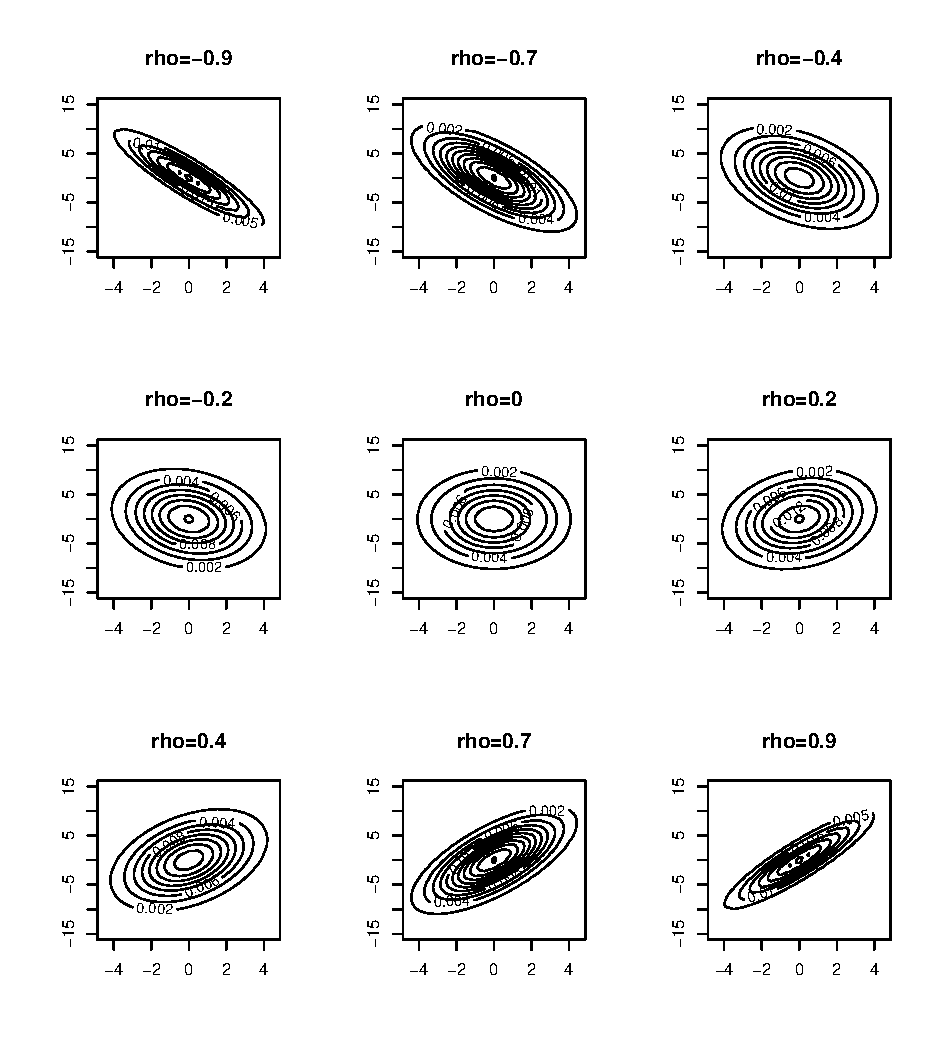
\includegraphics[scale=0.85]{normal_contorno.eps}
\caption[\textsl{Gr�fica de contorno para la distribuci�n normal bivariante}]{\textsl{Gr�fica de contorno para la distribuci�n normal bivariante con $\sigma_1=2$, $\sigma_2=5$ y diferentes valores de $\rho$.}}
\end{figure}

Un ejemplo de la distribuci�n normal bivariada que es muy com�n en la vida real son las variables peso y estatura en individuos de una ciudad. En la Figura 5.3 se muestra el histograma y gr�fica de dispersi�n de estas dos variables medidas en 200 habitantes de una ciudad. De los histogramas de las dos variables, podemos observar que cada variable puede ser descrita con la distribuci�n normal; y de la gr�fica de dispersi�n se observa una dependencia lineal entre estas dos variables dando indicio de una estructura de correlaci�n, y dado lo anterior, es necesario analizar las dos variables conjuntamente y la distribuci�n apropiada ser� la distribuci�n normal bivariada. Tambi�n es necesario se�alar que esta gr�fica es s�lo de car�cter exploratorio, m�s adelante se introducir�n pruebas estad�sticas acerca de si un conjunto de datos multivariados proviene de una distribuci�n normal multivariante.

\begin{figure}[!htb]
\centering
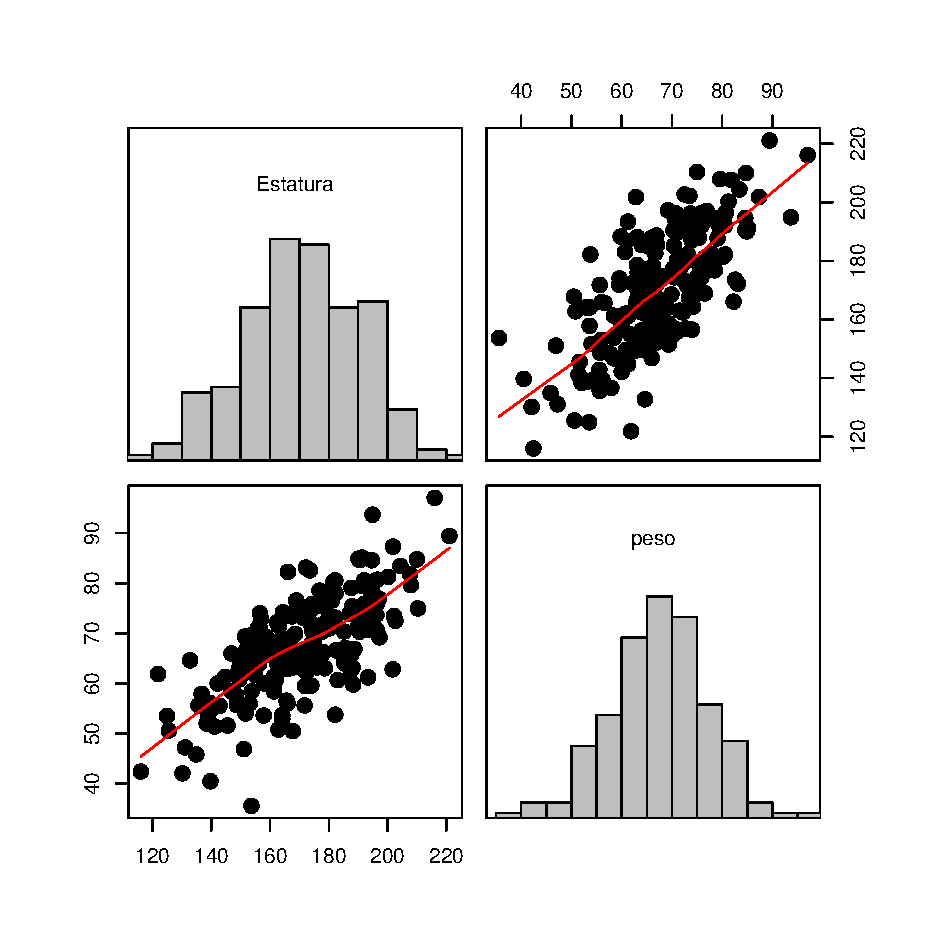
\includegraphics[scale=0.67]{normal_biva_ejemplo.eps}
\caption[\textsl{Histograma y gr�fica de dispersi�n de datos multivariantes}]{\textsl{Histograma y gr�fica de dispersi�n de las variables estatura y peso de 200 habitantes de una ciudad.}}
\end{figure}

Ahora, consideramos los datos de \citeasnoun{Student} donde se registran los incrementos de sue�o (en horas) en 10 pacientes con dos tipos de sedantes de hidrobromuro. Estos datos se muestran en la Tabla 5.2, donde los datos con signo negativo indican que se obtuvo una disminuci�n de sue�o en vez del incremento. Dado que los datos solo corresponden a 10 pacientes que constituyen una muestra peque�a, podemos utilizar las gr�ficas QQ plot para ver si la distribuci�n normal se ajusta bien a los dos grupos de datos. Esta gr�fica se muestra en la Figura 5.4.

\textbf{Nota:} cuando el vector aleatorio $\mathbf{X}$ es unidimensional, se reduce a una variable aleatoria, y su esperanza y matriz de varianzas y covarianzas se reducen a constantes, y si las denotan por $\mu$ y $\sigma^2$, la funci�n de densidad en (\ref{multinormal}) se reduce a la funci�n de densidad de una distribuci�n normal univariada.

\begin{table}\centering
\begin{tabular}{|c|cc|}\hline
Paciente&Sedante A&Sedante B\\\hline
1&  0.7  &  1.9\\
2& -1.6  &  0.8\\
3& -0.2  &  1.1\\
4& -1.2  &  0.1\\
5& -1.0  &  0.1\\
6&  3.4  &  4.4\\
7&  3.7  &  5.5\\
8&  0.8  &  1.6\\
9&  0.0  &  4.6\\
10&  2.0  & 1.4\\\hline
\end{tabular}\caption[\textsl{Datos incrementos de sue�o con dos tipos de sedantes}]{\textsl{Incrementos de sue�o (en horas) en 10 pacientes con dos tipos de sedantes de hidrobromuro.}}
\end{table}

\begin{figure}[!htb]
\centering
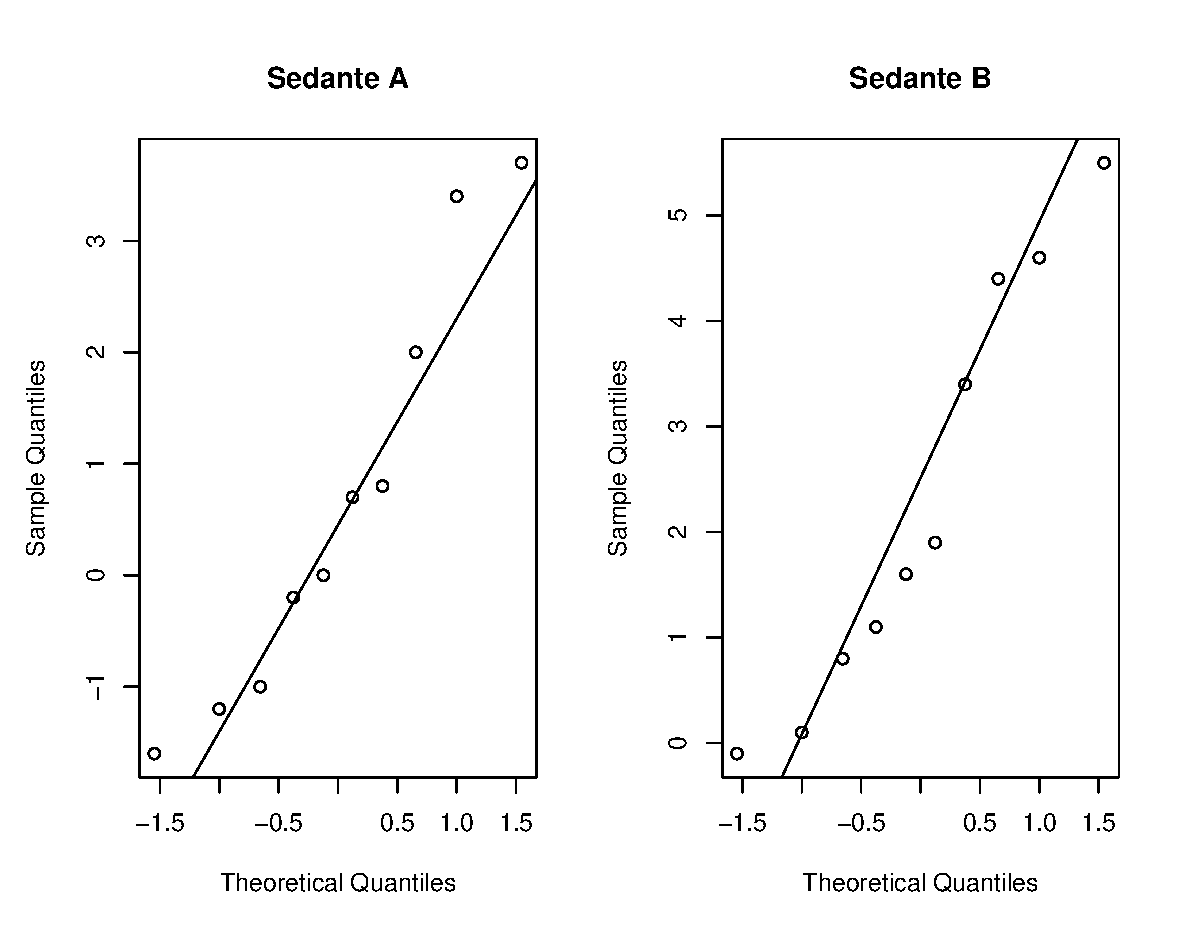
\includegraphics[scale=0.6]{sedante.eps}
\caption{\textsl{Gr�ficas QQ plot para los datos de la Tabla 5.2.}}
\end{figure}

Dado un vector aleatorio $\mathbf{X}\sim N_p(\boldsymbol{\mu},\mathbf{\Sigma})$, en el caso cuando $\boldsymbol{\mu}=\mathbf{0}$ y $\mathbf{\Sigma}=\mathbf{I}_p$, se dice que $\mathbf{X}$ tiene distribuci�n normal est�ndar multivariante. En este los componentes de $\mathbf{X}$ son variables aleatorias independientes, cada una con distribuci�n normal est�ndar.

\subsubsection{Caracter�stica de la funci�n de densidad de la distribuci�n $N_p$}
Dado que la distribuci�n normal multivariante es una generalizaci�n de la distribuci�n normal univariada, su funci�n de densidad tambi�n tiene comportamientos similares a los del caso univariado, como lo presenta el siguiente resultado.
\begin{Res}
Dado un vector aleatorio $\mathbf{X}\sim N_p(\boldsymbol{\mu},\mathbf{\Sigma})$, se tiene que
    \begin{enumerate}
    \item la funci�n de densidad es sim�trica con respecto a $\boldsymbol{\mu}$, esto es, $f(\boldsymbol{\mu}+\mathbf{a})=f(\boldsymbol{\mu}-\mathbf{a})$ para todo vector $\mathbf{a}\in\mathbb{R}^p$.
    \item la funci�n de densidad tiene un m�ximo en $\boldsymbol{\mu}$.
    \end{enumerate}
\end{Res}

\begin{proof}
    \begin{enumerate}
    \item Tenemos que
            \begin{align*}
                f(\boldsymbol{\mu}+\mathbf{a})&=|\mathbf{\Sigma}|^{-1/2}(2\pi)^{-p/2}\exp\{-\frac{1}{2}(\mathbf{a})'\mathbf{\Sigma}^{-1}(\mathbf{a})\}\\
                                              &=|\mathbf{\Sigma}|^{-1/2}(2\pi)^{-p/2}\exp\{-\frac{1}{2}(-\mathbf{a})'\mathbf{\Sigma}^{-1}(-\mathbf{a})\}\\
                                              &=f(\boldsymbol{\mu}-\mathbf{a})
            \end{align*}
    \item La matriz $\mathbf{\Sigma}$ es semidefinida positiva, y por consiguiente sus valores propios son no negativos; m�s aun, son todos positivos, pues $\mathbf{\Sigma}$ es invertible. De esta manera, los valores propios de $\mathbf{\Sigma}^{-1}$ tambi�n son todos positivos, de donde se concluye que tambi�n $\mathbf{\Sigma}^{-1}$ es semidefinida positiva; por consiguiente, para cualquier vector $\mathbf{x}$, se tiene que $(\mathbf{x}-\boldsymbol{\mu})'\mathbf{\Sigma}^{-1}(\mathbf{x}-\boldsymbol{\mu})\geq0$, entonces la funci�n de densidad de $\mathbf{X}$ tiene un m�ximo cuando $(\mathbf{x}-\boldsymbol{\mu})'\mathbf{\Sigma}^{-1}(\mathbf{x}-\boldsymbol{\mu})=0$, y esto se tiene cuando $\mathbf{x}=\boldsymbol{\mu}$, es decir, la funci�n de densidad de $\mathbf{X}$ tiene un m�ximo en $\boldsymbol{\mu}$.
    \end{enumerate}
\end{proof}


\subsubsection{Momentos y funci�n generadora de momentos de un vector aleatorio con distribuci�n $N_p$}
\begin{Res}
\index{Distribuci�n!normal multivariante!propiedades}Si $\mathbf{Z}=(Z_1,\cdots,Z_p)'\sim N_p(\mathbf{0},\mathbf{I}_p)$, entonces las variables $Z_1$, $\cdots$, $Z_p$ son independientes con $Z_i\sim N(0,1)$. Y $E(\mathbf{Z})=\mathbf{0}$, $Var(\mathbf{Z})=\mathbf{I}_p$ y $M_{\mathbf{Z}}(\mathbf{t})=e^{\mathbf{t}'\mathbf{t}/2}$
\end{Res}
\begin{proof}
Entonces por la definici�n de distribuci�n multivariante, se tiene que la funci�n de densidad $\mathbf{Z}$ est� dada por
\begin{align*}
f(\mathbf{z})=f(z_1,\cdots,z_p)&=(2\pi)^{-p/2}\exp\left\{-\frac{1}{2}\mathbf{z}'\mathbf{z}\right\}\\
&=(2\pi)^{-p/2}\exp\left\{-\frac{1}{2}\sum_{i=1}^pz_i^2\right\}\\
&=\prod_{i=1}^Pr(2\pi)^{-1/2}\exp\left\{-\frac{1}{2}z_i^2\right\}\\
\end{align*}

donde cada t�rmino $(2\pi)^{-1/2}\exp\left\{-\frac{1}{2}z_i^2\right\}$ corresponde a la funci�n de densidad de una distribuci�n $N(0,1)$. As�, podemos ver que los componentes de $\mathbf{Z}$, $Z_1$, $\cdots$, $Z_p$ son variables aleatorias independientes e id�nticamente distribuidas con distribuci�n normal est�ndar. Y dadas las propiedades en t�rminos de la esperanza y la varianza de esta distribuci�n, es f�cil ver que $E(\mathbf{Z})=\mathbf{0}$ y $Var(\mathbf{Z})=\mathbf{I}_p$. Adicionalmente, la funci�n generadora de momentos de $\mathbf{Z}$ se puede calcular como
\begin{align*}
M_{\mathbf{Z}}(\mathbf{t})=E(e^{\mathbf{Z}'\mathbf{t}})=\prod_{i=1}^pE(e^{Z_it_i})=\prod_{i=1}^pM_{Z_i}(t_i)=e^{\mathbf{t}'\mathbf{t}/2}
\end{align*}
\end{proof}

Utilizando el anterior resultado con respecto a la distribuci�n normal est�ndar multivariante, tenemos las siguientes propiedades para cualquier distribuci�n normal multivariante.

\begin{Res} Si $\mathbf{X}$ es un vector aleatorio con distribuci�n $N_p(\boldsymbol{\mu},\mathbf{\Sigma})$, entonces tenemos que\index{Distribuci�n!normal multivariante!propiedades}
\begin{enumerate}
\item Para cualquier matriz $A$ de dimensi�n $r\times p$ y vector $b$ de dimensi�n $r\times1$, se tiene que $A\mathbf{X}+b\sim N_{r}(A\boldsymbol{\mu}+b,A\mathbf{\Sigma} A)'$. En particular, para cualesquiera constantes $c_1$, $\cdots$, $c_p$, se tiene que $\sum_{i=1}^pc_iX_i$ tiene distribuci�n normal.
\item $E(\mathbf{X})=\boldsymbol{\mu}$ y $Var(\mathbf{X})=\mathbf{\Sigma}$.
\item La funci�n generadora de momentos de $\mathbf{X}$ est� dada por
    \begin{equation}\label{mgt}
    M_{\mathbf{X}}(t)=\exp\{\boldsymbol{\mu}'\mathbf{t}+\frac{\mathbf{t}'\mathbf{\Sigma}\mathbf{t}}{2}\}.
    \end{equation}
    Adem�s la funci�n generadora de momentos caracteriza la distribuci�n de $\mathbf{X}$.
\item Por ser la matriz $\mathbf{\Sigma}$ semidefinida positiva, existe una matriz $A$ sim�trica cuadrada con $\mathbf{\Sigma}=AA$, y el vector aleatorio $A^{-1}(\mathbf{X}-\boldsymbol{\mu})$ tiene distribuci�n $N_p(\mathbf{0},\mathbf{I}_p)$.
\item Cualquier subvector de $\mathbf{X}$ tambi�n tiene distribuci�n normal multivariante.
\item se tiene que la variable aleatoria $(\mathbf{X}-\boldsymbol{\mu})'\mathbf{\Sigma}^{-1}(\mathbf{X}-\boldsymbol{\mu})$ es decir, la distancia de Mahalanobis entre $\mathbf{X}$ y $\boldsymbol{\mu}$, tiene distribuci�n Ji-cuadrado con $p$ grados de libertad.
\end{enumerate}
\end{Res}

\begin{proof}
La demostraci�n de estas propiedades se basa principalmente en el hecho de que dado un vector $\mathbf{Z}\sim N(\mathbf{0},\mathbf{I}_p)$, entonces mediante el teorema de transformaci�n, se puede encontrar que la funci�n de densidad del vector $\mathbf{\Sigma}^{1/2}\mathbf{Z}+\boldsymbol{\mu}$ est� dada por
\begin{equation*}
f(\mathbf{x})=|\mathbf{\Sigma}|^{-1/2}(2\pi)^{-p/2}\exp\left\{-\frac{1}{2}(\mathbf{x}-\boldsymbol{\mu})'\mathbf{\Sigma}^{-1}(\mathbf{x}-\boldsymbol{\mu})\right\}
\end{equation*}

de donde podemos ver que $\mathbf{X}\sim N_p(\boldsymbol{\mu},\mathbf{\Sigma})$, y en conclusi�n $\mathbf{X}$ se puede escribir como $\mathbf{X}=\mathbf{\Sigma}^{1/2}\mathbf{Z}+\boldsymbol{\mu}$ donde $\mathbf{Z}\sim N(\mathbf{0},\mathbf{I}_p)$. Usando este hecho podemos probar las propiedades enunciadas como sigue:

\begin{enumerate}
\item Para demostrar este resultado, se usa el hecho de que la funci�n generadora de momentos caracteriza la distribuci�n. Veamos que la funci�n generadora de momentos de $A\mathbf{X}+b$ es de la forma de (\ref{mgt}). Tenemos que
    \begin{align*}
    M_{A\mathbf{X}+b}(\mathbf{t})&=E(e^{(A\mathbf{X}+b)'\mathbf{t}})
                                 =E(e^{\mathbf{X}'A'\mathbf{t}})e^{b'\mathbf{t}}
                                 =M_{\mathbf{X}}(A't)e^{b'\mathbf{t}}\\
                                 &=\exp\{\boldsymbol{\mu}'A'\mathbf{t}+\frac{(A'\mathbf{t})'\mathbf{\Sigma} A'\mathbf{t}}{2}\}\exp\{b'\mathbf{t}\}\\
                                 &=\exp\{(\boldsymbol{\mu}'A'+b')t+\frac{\mathbf{t}'A\mathbf{\Sigma} A'\mathbf{t}}{2}\}.
    \end{align*}
    Esta funci�n es de la forma de (\ref{mgt}), de donde se concluye que $A\mathbf{X}+b\sim N_{r}(A\boldsymbol{\mu}+b,A\mathbf{\Sigma} A)'$.
\item Se tiene trivialmente usando conjuntamente la parte 1, los Resultados 5.1.2, 5.2.3 y la parte (d) del Resultado 5.1.4.
\item Tenemos que
    \begin{equation*}
    M_{\mathbf{X}}(\mathbf{t})=E(e^{(\mathbf{\Sigma}^{1/2}\mathbf{Z}+\boldsymbol{\mu})'\mathbf{t}})
    =M_{\mathbf{Z}}(\mathbf{\Sigma}^{1/2}\mathbf{t})e^{\boldsymbol{\mu}'\mathbf{t}}
    =e^{(\mathbf{\Sigma}^{1/2}\mathbf{t})'\mathbf{\Sigma}^{1/2}\mathbf{t}/2}e^{\boldsymbol{\mu}'\mathbf{t}}
    =e^{\boldsymbol{\mu}'\mathbf{t}+\mathbf{t}'\mathbf{\Sigma}\mathbf{t}/2}
    \end{equation*}
\item Trivial usando el resultado anterior.
\item Ilustrando la demostraci�n suponiendo que si $\mathbf{X}$ se puede dividir en dos subvectores, entonces cada subvector tiene distribuci�n normal. Esto es, si
    \begin{equation*}
    \mathbf{X}=
    \left(
      \begin{array}{c}
        \mathbf{X}_1 \\
        \mathbf{X}_2 \\
      \end{array}
    \right)
    \end{equation*}

    entonces particionando adecuadamente $\mathbf{\Sigma}$, $\boldsymbol{\mu}$ y $\mathbf{Z}$, $\mathbf{X}=\mathbf{\Sigma}^{1/2}\mathbf{Z}+\boldsymbol{\mu}$ se puede escribir como
    \begin{equation*}
    \mathbf{X}=
    \left(
      \begin{array}{c}
        \mathbf{X}_1 \\
        \mathbf{X}_2 \\
      \end{array}
    \right)=\left(\begin{array}{cc}
              \mathbf{\Sigma}^{1/2}_{11} & \mathbf{\Sigma}^{1/2}_{12} \\
              \mathbf{\Sigma}^{1/2}_{21}  & \mathbf{\Sigma}^{1/2}_{22}
            \end{array}\right)
    \left(
      \begin{array}{c}
        \mathbf{Z}_1 \\
        \mathbf{Z}_2 \\
      \end{array}
    \right)+\left(
      \begin{array}{c}
        \boldsymbol{\mu}_1 \\
        \boldsymbol{\mu}_2 \\
      \end{array}
    \right)\end{equation*}

    Y por consiguiente $\mathbf{X}_1=(\mathbf{\Sigma}^{1/2}_{11},\mathbf{\Sigma}^{1/2}_{12})(\mathbf{Z}_1,\mathbf{Z}_2)'+\boldsymbol{\mu}_1$. La aplicaci�n del numeral 3 lleva a la conclusi�n de que el subvector $\mathbf{X}_1$ tiene distribuci�n normal. De manera an�loga se encuentra que el subvector $\mathbf{X}_2$ tambi�n tiene distribuci�n normal.
\item Utilizando, de nuevo, $\mathbf{X}=\mathbf{\Sigma}^{1/2}\mathbf{Z}+\boldsymbol{\mu}$, tenemos que
    \begin{equation*}
    (\mathbf{X}-\boldsymbol{\mu})'\mathbf{\Sigma}^{-1}(\mathbf{X}-\boldsymbol{\mu})=\mathbf{Z}'\mathbf{Z}=\sum_{i=1}^pZ_i^2
    \end{equation*}

    Utilizando la definici�n de la distribuci�n $\chi^2$ y el hecho de que las variables $Z_1$, $\cdots$, $Z_p$ son independientes, cada uno con distribuci�n normal est�ndar, tenemos que $(\mathbf{X}-\boldsymbol{\mu})'\mathbf{\Sigma}^{-1}(\mathbf{X}-\boldsymbol{\mu})\sim\chi^2_p$.
\end{enumerate}
\end{proof}

\newpage

En la propiedad 4, se debe hallar la ra�z cuadrada de la matriz $\mathbf{\Sigma}$. Este c�lculo se puede llevar a cabo usando la descomposici�n $\mathbf{\Sigma}=QDQ'$, siendo $Q$ la matriz que contiene los vectores propios ortonormales de $\mathbf{\Sigma}$, y $\mathbf{D}$ la matriz diagonal que contiene los valores propios de $\mathbf{\Sigma}$. Al definir $A=QD^{1/2}Q'$, se tiene que $\mathbf{\Sigma}=AA$. El siguiente c�digo en R permite encontrar la matriz $A$
\begin{verbatim}
> p<-3
> gama<-matrix(c(6,1,-1,1,5,0,-1,0,4),p,p)
> Q<-eigen(gama)$vectors
> D<-diag(eigen(gama)$values)
> A<-Q%*%sqrt(D)%*%t(Q)
\end{verbatim}

La propiedad 5 del resultado anterior, establece que si un vector $(X_1,X_2)'$ tiene distribuci�n normal bivariada, entonces tanto $X_1$ como $X_2$ tienen distribuci�n normal univariante. Sin embargo, el rec�proco no es cierto, es decir, dadas dos variables $X_1$ y $X_2$, cada una con distribuci�n normal, el vector $(X_1,X_2)'$ no necesariamente tiene distribuci�n normal bivariada. Pero si $X_1$ y $X_2$ son variables independientes, entonces el vector $(X_1,X_2)'$ s� tiene distribuci�n normal bivariada (Ejercicio 5.8).

\begin{Res}
\index{Distribuci�n!normal multivariante!propiedades}Sean vectores aleatorios $\mathbf{X}_1$, $\cdots$, $\mathbf{X}_n$ independientes y distribuidos como $N_p(\boldsymbol{\mu}_i,\mathbf{\Sigma}_i)$, entonces, se tiene que para constantes $c_1$, $\cdots$, $c_n$, se tiene que el vector aleatorio $\mathbf{Y}=\sum_{i=1}^nc_i\mathbf{X_i}$ se distribuye como\\ $N_p(\sum_{i=1}^nc_i\boldsymbol{\mu}_i,\sum_{i=1}^nc_i\mathbf{\Sigma}_i)$
\end{Res}
\begin{proof}
Se hace uso de la funci�n generadora de momentos, tenemos que
\begin{align}
m_{\mathbf{Y}}(\mathbf{t})&=m_{\sum_{i=1}^nc_i\mathbf{X_i}}(\mathbf{t})\\
&=\prod_{i=1}^nm_{\mathbf{X}_i}(c_i\mathbf{t})\ \ \ \ \ \text{Resultado 5.1.7.}\\
&=\prod_{i=1}^n\exp\{c_i\boldsymbol{\mu}_i'\mathbf{t}+\frac{c_i^2\mathbf{t}'\mathbf{\Sigma}_i\mathbf{t}}{2}\}\\
&=\exp\{\sum_{i=1}^n\boldsymbol{\mu}_i'\mathbf{t}+\frac{\mathbf{t}'\sum_{i=1}^nc_i\mathbf{\Sigma}_i\mathbf{t}}{2}\},
\end{align}
de donde se concluye que $\mathbf{Y}\sim N_p(\sum_{i=1}^nc_i\boldsymbol{\mu}_i,\sum_{i=1}^nc_i\mathbf{\Sigma}_i)$
\end{proof}
N�tese que en el anterior resultado, cuando son los vectores aleatorios $\mathbf{X}_1$, $\cdots$, $\mathbf{X}_n$ son id�nticamente distribuidos, con distribuci�n  $N_p(\boldsymbol{\mu},\mathbf{\Sigma})$, se tiene que el promedio definido como
\begin{equation}\label{barX}
\bar{\mathbf{X}}=\frac{1}{n}\sum_{i=1}^n\mathbf{X}_i
\end{equation}
tiene distribuci�n $N_p(\boldsymbol{\mu},\frac{1}{n}\mathbf{\Sigma})$.

Finalmente, consideramos la distribuci�n condicional dentro de la distribuci�n normal multivariante. Suponga que $\mathbf{X}\sim N_p(\boldsymbol{\mu},\mathbf{\Sigma})$, y dividimos el vector $\mathbf{X}$ como $\mathbf{X}=(\mathbf{X}_1',\mathbf{X}_2')'$ donde $\mathbf{X}_1$ y $\mathbf{X}_2$ son vectores de dimensi�n $p_1$ y $p_2$, respectivamente, con $p_1+p_2=p$. Esta divisi�n tambi�n induce a una divisi�n en el vector de medias $\boldsymbol{\mu}$ y la matriz de varianzas $\mathbf{\Sigma}$ como $\boldsymbol{\mu}=(\boldsymbol{\mu}_1',\boldsymbol{\mu}_2')'$ y
\begin{equation*}
\mathbf{\Sigma}=\begin{pmatrix}
\mathbf{\Sigma}_{11}&\mathbf{\Sigma}_{12}\\
\mathbf{\Sigma}_{21}&\mathbf{\Sigma}_{22}
\end{pmatrix}
\end{equation*}

donde $\boldsymbol{\mu}_1$ y $\boldsymbol{\mu}_2$ son los vectores de medias de $\mathbf{X}_1$ y $\mathbf{X}_2$; $\mathbf{\Sigma}_{11}$ y $\mathbf{\Sigma}_{22}$ son las matrices de varianzas y covarianzas de $\mathbf{X}_1$ y $\mathbf{X}_2$; y $\mathbf{\Sigma}_{12}=\mathbf{\Sigma}_{21}'$ es la matriz que contiene las covarianzas entre cada componente de $\mathbf{X}_1$ y cada componente de $\mathbf{X}_2$. En el siguiente resultado mostramos la distribuci�n de $\mathbf{X}_1$ dado $\mathbf{X}_2$ cuando el vector completo $\mathbf{X}$ tiene distribuci�n normal multivariante.

\begin{Res}
Dada la divisi�n enunciada anteriormente, si $\mathbf{X}\sim N_p(\boldsymbol{\mu},\mathbf{\Sigma})$, entonces la distribuci�n de $\mathbf{X}_1$ condicionada a que $\mathbf{X}_2$ tome el valor $\mathbf{x}_2$ es normal con esperanza\index{Distribuci�n!normal multivariante!esperanza condicional}
\begin{equation*}
E(\mathbf{X}_1|\mathbf{X}_2=\mathbf{x}_2)=\boldsymbol{\mu}_1+\mathbf{\Sigma}_{12}\mathbf{\Sigma}^{-1}_{22}(\mathbf{x}_2-\boldsymbol{\mu}_2)
\end{equation*}

y matriz de varianzas y covarianzas
\begin{equation*}
Var(\mathbf{X}_1|\mathbf{X}_2=\mathbf{x}_2)=\mathbf{\Sigma}_{11}-\mathbf{\Sigma}_{12}\mathbf{\Sigma}^{-1}_{22}\mathbf{\Sigma}_{21}
\end{equation*}
\end{Res}

\begin{proof}
La prueba del resultado consiste en encontrar la funci�n de densidad de $\mathbf{X}_1$ dado $\mathbf{X}_2=\mathbf{x}_2$. Tenemos que
\begin{align*}
f(\mathbf{x}_1|\mathbf{x}_2)&=\dfrac{f_{\mathbf{X}_1,\mathbf{X}_2}(\mathbf{x}_1,\mathbf{x}_2)}{f_{\mathbf{X}_2}(\mathbf{x}_2)}\\
&=\dfrac{|\mathbf{\Sigma}|^{-1/2}(2\pi)^{-p/2}
\exp\{-\frac{1}{2}(\mathbf{x}-\boldsymbol{\mu})'\mathbf{\Sigma}^{-1}(\mathbf{x}-\boldsymbol{\mu})\}}
{|\mathbf{\Sigma}_{22}|^{-1/2}(2\pi)^{-p_2/2}\exp\{-\frac{1}{2}(\mathbf{x}_2-\boldsymbol{\mu}_2)'\mathbf{\Sigma}_{22}^{-1}(\mathbf{x}_2-\boldsymbol{\mu}_2)\}}
\end{align*}

Usando la propiedad de una matriz particionada con respecto al determinante, tenemos que $|\mathbf{\Sigma}|=|\mathbf{\Sigma}_{22}||\mathbf{\Sigma}_{11}-\mathbf{\Sigma}_{12}\mathbf{\Sigma}_{22}^{-1}\mathbf{\Sigma}_{21}|$ y $p_1+p_2=p$, tenemos que
\begin{align*}
f(\mathbf{x}_1|\mathbf{x}_2)&=|\mathbf{\Sigma}_{11}-\mathbf{\Sigma}_{12}\mathbf{\Sigma}_{22}^{-1}\mathbf{\Sigma}_{21}|^{-1/2}(2\pi)^{-p_1/2}\\
&\times\exp\left\{-\frac{1}{2}\left[(\mathbf{x}-\boldsymbol{\mu})'\mathbf{\Sigma}^{-1}(\mathbf{x}-\boldsymbol{\mu})-(\mathbf{x}_2-\boldsymbol{\mu}_2)'\mathbf{\Sigma}_{22}^{-1}(\mathbf{x}_2-\boldsymbol{\mu}_2)\right]\right\}
\end{align*}

Ahora consideramos el t�rmino dentro del exponente $(\mathbf{x}-\boldsymbol{\mu})'\mathbf{\Sigma}^{-1}(\mathbf{x}-\boldsymbol{\mu})-(\mathbf{x}_2-\boldsymbol{\mu}_2)'\mathbf{\Sigma}_{22}^{-1}(\mathbf{x}_2-\boldsymbol{\mu}_2)$, usando la propiedad de una matriz particionada con respecto a la inversa, tenemos que
\begin{equation*}
\mathbf{\Sigma}^{-1}=\begin{pmatrix}
\mathbf{B}^{-1}&-\mathbf{B}^{-1}\mathbf{\Sigma}_{12}\mathbf{\Sigma}_{22}^{-1}\\
-\mathbf{\Sigma}_{22}^{-1}\mathbf{\Sigma}_{21}\mathbf{B}^{-1}&\mathbf{\Sigma}_{22}^{-1}+\mathbf{\Sigma}_{22}^{-1}\mathbf{\Sigma}_{21}\mathbf{B}^{-1}\mathbf{\Sigma}_{12}\mathbf{\Sigma}_{22}^{-1}
\end{pmatrix}
\end{equation*}

con $\mathbf{B}=\mathbf{\Sigma}_{11}-\mathbf{\Sigma}_{12}\mathbf{\Sigma}^{-1}_{22}\mathbf{\Sigma}_{21}$. Desarrollando los productos matriciales, se puede ver que

\newpage

\begin{align*}
&\ \ \ \ \ (\mathbf{x}-\boldsymbol{\mu})'\mathbf{\Sigma}^{-1}(\mathbf{x}-\boldsymbol{\mu})-(\mathbf{x}_2-\boldsymbol{\mu}_2)'\mathbf{\Sigma}_{22}^{-1}(\mathbf{x}_2-\boldsymbol{\mu}_2)\\
&=
(\mathbf{x}_1-\boldsymbol{\mu}_1)'\mathbf{B}^{-1}(\mathbf{x}_1-\boldsymbol{\mu}_1)-(\mathbf{x}_1-\boldsymbol{\mu}_1)'\mathbf{B}^{-1}\mathbf{\Sigma}_{12}\mathbf{\Sigma}_{22}^{-1}(\mathbf{x}_2-\boldsymbol{\mu}_2)\\
&\ \ \ \ \ \ \ \ \ \ \ \ \ \ \ -(\mathbf{x}_2-\boldsymbol{\mu}_2)'\mathbf{\Sigma}^{-1}_{22}\mathbf{\Sigma}_{21}\mathbf{B}^{-1}(\mathbf{x}_1-\boldsymbol{\mu}_1)\\
&\ \ \ \ \ \ \ \ \ \ \ \ \ \ \ \ \ \ \ \ \ \ \ \ \ +
(\mathbf{x}_2-\boldsymbol{\mu}_2)'\mathbf{\Sigma}^{-1}_{22}\mathbf{\Sigma}_{21}\mathbf{B}^{-1}\mathbf{\Sigma}_{12}\mathbf{\Sigma}^{-1}_{22}(\mathbf{x}_2-\boldsymbol{\mu}_2)\\
& =\left[(\mathbf{x}_1-\boldsymbol{\mu}_1)'-(\mathbf{x}_2-\boldsymbol{\mu}_2)'\mathbf{\Sigma}^{-1}_{22}\mathbf{\Sigma}_{21}\right]\mathbf{B}^{-1}(\mathbf{x}_1-\boldsymbol{\mu}_1)\\
&\ \ \ \ \ \ \ \ \ \ \ \ \ \ -\left[(\mathbf{x}_1-\boldsymbol{\mu}_1)'-(\mathbf{x}_2-\boldsymbol{\mu}_2)'\mathbf{\Sigma}^{-1}_{22}\mathbf{\Sigma}_{21}\right]\mathbf{B}^{-1}\mathbf{\Sigma}_{12}\mathbf{\Sigma}^{-1}_{22}(\mathbf{x}_2-\boldsymbol{\mu}_2)\\
&=\left[(\mathbf{x}_1-\boldsymbol{\mu}_1)'-(\mathbf{x}_2-\boldsymbol{\mu}_2)'\mathbf{\Sigma}^{-1}_{22}\mathbf{\Sigma}_{21}\right]\mathbf{B}^{-1}\left[\mathbf{x}_1-\boldsymbol{\mu}_1-\mathbf{\Sigma}_{12}\mathbf{\Sigma}^{-1}_{22}(\mathbf{x}_2-\boldsymbol{\mu}_2)\right]\\
&=\left[\mathbf{x}_1-\boldsymbol{\mu}_1-\mathbf{\Sigma}_{12}\mathbf{\Sigma}^{-1}_{22}(\mathbf{x}_2-\boldsymbol{\mu}_2)\right]'\mathbf{B}^{-1}\left[\mathbf{x}_1-\boldsymbol{\mu}_1-\mathbf{\Sigma}_{12}\mathbf{\Sigma}^{-1}_{22}(\mathbf{x}_2-\boldsymbol{\mu}_2)\right].
\end{align*}

Utilizando lo anterior, tenemos que la funci�n de densidad de $\mathbf{X}_1$ dado $\mathbf{X}_2=\mathbf{x}_2$ es
\begin{multline*}
f(\mathbf{x}_1|\mathbf{x}_2)=|\mathbf{B}|^{-1/2}
(2\pi)^{-p_1/2}\\\exp\left\{-\frac{1}{2}\left(\mathbf{x}_1-\boldsymbol{\mu}_1-\mathbf{\Sigma}_{12}\mathbf{\Sigma}^{-1}_{22}(\mathbf{x}_2-\boldsymbol{\mu}_2)\right)'\mathbf{B}^{-1}\left(\mathbf{x}_1-\boldsymbol{\mu}_1-\mathbf{\Sigma}_{12}\mathbf{\Sigma}^{-1}_{22}(\mathbf{x}_2-\boldsymbol{\mu}_2)\right)\right\}
\end{multline*}
con $\mathbf{B}=\mathbf{\Sigma}_{11}-\mathbf{\Sigma}_{12}\mathbf{\Sigma}^{-1}_{22}\mathbf{\Sigma}_{21}$. Esta funci�n coincide con la funci�n de densidad de una distribuci�n normal con media y $\boldsymbol{\mu}_1+\mathbf{\Sigma}_{12}\mathbf{\Sigma}^{-1}_{22}(\mathbf{x}_2-\boldsymbol{\mu}_2)$ y matriz de varianzas $\mathbf{\Sigma}_{11}-\mathbf{\Sigma}_{12}\mathbf{\Sigma}^{-1}_{22}\mathbf{\Sigma}_{21}$.
\end{proof}

Observamos que cuando no existe ninguna relaci�n lineal entre $\mathbf{X}_1$ y $\mathbf{X}_2$, $\mathbf{\Sigma}_{12}=0$ y como consecuencia $E(\mathbf{X}_1|\mathbf{X}_2=\mathbf{x}_2)=E(\mathbf{X}_1)$ y $Var(\mathbf{X}_1|\mathbf{X}_2=\mathbf{x}_2)=Var(\mathbf{X}_1)$, esto es, el condicionamiento sobre $\mathbf{X}_2=\mathbf{x}_2$ no afecta la distribuci�n del vector $\mathbf{X}_1$.

\subsection{Distribuci�n Wishart}

Al igual que la definici�n de un vector aleatorio, se puede definir una matriz aleatoria como sigue
\begin{Defi}
Una matriz $A$ de dimensi�n $p\times q$, cuyos elementos son variables aleatorias se llama una matriz aleatoria.\index{Distribuci�n!Wishart}
\end{Defi}

La teor�a asociada a las matrices aleatorias es bastante complicada, los lectores interesados pueden consultar \citeasnoun{Gupta} para una revisi�n detallada de este aspecto. En el presente libro s�lo se introducir� la distribuci�n Wishart con el fin de desarrollar la teor�a de inferencia acerca de la matriz de varianzas y covarianzas de una distribuci�n normal multivariante\footnote{Cuando se desea estimar la matriz de varianzas y covarianzas de una distribuci�n normal multivariante, el estimador tambi�n debe ser de forma matricial. En el pr�ximo cap�tulo se ver� que la distribuci�n de este estimador est� asociada con la distribuci�n Wishart, y evaluaremos la calidad del estimador usando las propiedades de esa distribuci�n.}, mas no estamos considerando datos en forma matricial que puedan ser descritos con la distribuci�n Wishart.

\begin{Defi}
Una matriz aleatoria $A$ cuadrada de dimensi�n $p\times p$ tiene distribuci�n Wishart con matriz de par�metros $\Sigma$ y grados de libertad $n$, si la funci�n de densidad de $A$ est� dada por
\begin{equation}
f(A)=\dfrac{|A|^{(n-p-1)/2}}{2^{np/2}|\Sigma|^{n/2}\mathbf{\Sigma}_Pr(\frac{n}{2})}\exp\left\{-\frac{1}{2}tr(\Sigma^{-1}A)\right\}
\end{equation}
donde $\Sigma$ es una matriz $p\times p$ definida positiva, $n$ es un entero positivo con $n\geq p$, y $\mathbf{\Sigma}_Pr(\cdot)$ es la funci�n gamma multivariada definida como
\begin{equation*}
\mathbf{\Sigma}_Pr(k)=\pi^{p(p-1)/4}\prod_{i=1}^p\mathbf{\Sigma}(\frac{2k+1-i}{2}).
\end{equation*}
La notaci�n para esta distribuci�n es $A\sim W(n,\Sigma)$.
\end{Defi}
La distribuci�n Wishart es la versi�n multivariante de la distribuci�n Ji-cuadrado, cuando $p=1$, $A$ se reduce a un vector aleatorio y cuando $\Sigma=1$, la anterior expresi�n se reduce a la funci�n de densidad de una distribuci�n $\chi^2_n$.

Existe otra definici�n equivalente para la distribuci�n Wishart, que afirma:
\begin{Defi}
Sea $\mathbf{X}_1$, $\cdots$, $\mathbf{X}_n$ vectores aleatorios independientes e id�nticamente distribuidos como $N_p(\boldsymbol{0},\mathbf{\Sigma})$, entonces la matriz $\sum_{i=1}^n\mathbf{X}_i\mathbf{X}_i'$ tiene distribuci�n Wishart con matriz de par�metros $\Sigma$ y grados de libertad $n$.
\end{Defi}

En el siguiente resultado se enuncian algunas propiedades de la distribuci�n Wishart.
\begin{Res}
Si $A\sim W(n,\Sigma)$, entonces\index{Distribuci�n!Wishart!propiedades}
\begin{enumerate}
    \item $E(A)=n\Sigma$
    \item para cualquier matriz $B$ de constantes de dimensi�n $r\times p$, se tiene que $BAB'\sim W(n,B\mathbf{\Sigma} B')$
    \item la funci�n caracter�stica est� dada por $C_A(\Theta)=|I_p-2i\Theta\Sigma|^{-n/2}$ para $\Theta$ matriz de dimensi�n $p\times p$
\end{enumerate}
\end{Res}

\begin{proof}
La demostraci�n har� uso de la definici�n 5.3.3.
\begin{enumerate}
    \item Tenemos que
        \begin{align*}
            E(A)=E(\sum_{i=1}^n\mathbf{X}_i\mathbf{X}_i')
                =\sum_{i=1}^nE(\mathbf{X}_i\mathbf{X}_i')
                =\sum_{i=1}^nVar(\mathbf{X}_i)
                =\sum_{i=1}^n\mathbf{\Sigma}
                =n\mathbf{\Sigma}
        \end{align*}
    \item Tenemos que $BAB'=B\sum_{i=1}^n\mathbf{X}_i\mathbf{X}_i'B'=\sum_{i=1}^nB\mathbf{X}_i\mathbf{X}_i'B'=\sum_{i=1}^nB\mathbf{X}_i(B\mathbf{X}_i)'$. Por el Resultado 5.2.4 parte 1, se tiene que $B\mathbf{X}_i\sim N_p(\boldsymbol{0},B\Sigma B')$; adem�s, $Cov(B\mathbf{X}_i,B\mathbf{X}_j)=BCov(\mathbf{X}_i,\mathbf{X}_j)B'=B\mathbf{0}B'=\mathbf{0}$, de donde se concluye que los vectores $B\mathbf{X}_1$, $\cdots$, $B\mathbf{X}_n$ son independientes. Entonces por la definici�n 5.3.3, se tiene que $\sum_{i=1}^nB\mathbf{X}_i(B\mathbf{X}_i)'\sim W(n,B\Sigma B')$, y el resultado queda demostrado.
\end{enumerate}
\end{proof}

\newpage

\begin{Res}
Sean $A_1$, $\cdots$, $A_n$ matrices aleatorias independientes donde $A_i\sim W(n_i,\Sigma)$ para $i=1,\cdots,n$, entonces $\sum_{i=1}^nA_i\sim W(\sum_{i=1}^nn_i,\Sigma)$.\index{Distribuci�n!Wishart!propiedades}
\end{Res}
\begin{proof}
La demostraci�n har� uso de la funci�n caracter�stica de la distribuci�n Wishart. Luego, tenemos que
\begin{align*}
     C_{\sum_{i=1}^nA_i}(\Theta)&=\prod_{i=1}^nC_{A_i}(\Theta)\ \ \ \ \ \text{(por la independencia)}\\
                                &=\prod_{i=1}^n|I_p-2i\Theta\Sigma|^{-n_i/2}=|I_p-2i\Theta\Sigma|^{-\sum_{i=1}^nn_i/2},
\end{align*}
de donde se concluye que $\sum_{i=1}^nA_i\sim W(\sum_{i=1}^nn_i,\Sigma)$.
\end{proof}

\subsection{Distribuci�n $T^2$ de Hotelling}
La distribuci�n $T^2$ de Hotelling\index{Distribuci�n!T2 de Hotelling} debe su nombre al estad�stico americano Harold Hotelling y es muy �til en la teor�a de la inferencia estad�stica multivariada. Aunque esta distribuci�n se define para variables aleatorias y no para vectores aleatorios, la raz�n por la que presentamos esta distribuci�n en este cap�tulo del libro es que la distribuci�n $T^2$ de Hotelling est� �ntimamente ligada con la distribuci�n normal multivariante, como se enuncia a continuaci�n.

\begin{figure}[!htb]
\centering
\includegraphics[bb=0 0 211 288, scale=0.5]{Hotelling.jpg}
\caption{\textsl{Harold Hotelling (1895-1973)}.}
\end{figure}

\begin{Defi}
Dado un vector aleatorio $\mathbf{X}\sim N_p(\boldsymbol{\mu},\mathbf{\Sigma})$, y sea $\mathbf{W}$ una matriz aleatoria con distribuci�n $W(\mathbf{\Sigma},n-1)$ para alg�n entero positivo $n$, si $\mathbf{W}$ es independiente de $\mathbf{X}$, entonces
\begin{equation*}
T^2=(\mathbf{X}-\boldsymbol{\mu})'\left(\frac{\mathbf{W}}{n-1}\right)^{-1}(\mathbf{X}-\boldsymbol{\mu})
\end{equation*}

tiene distribuci�n $T^2$ de Hotelling de grados de libertad $p$ y $n-1$.
\end{Defi}

\section{Ejercicios}
\begin{enumerate}[5.1]

\item Verificar las probabilidades y las esperanzas del Ejemplo 5.1.1.

\item Demuestre el Resultado 5.1.8.

\item Diga dos ejemplos en la vida real de variables que deben ser analizadas conjuntamente debido a la presencia de  estructuras de dependencia lineal.

\item Dado un vector aleatorio $\mathbf{X}=(X_1,X_2)'$ con $X_1\sim N(1,4)$ y $X_2$ con distribuci�n exponencial de media 5, y $Cov(X_1,X_2)=2$, encuentre
    \begin{enumerate}[(a)]
    \item La esperanza, la matriz de varianzas y covarianzas y la matriz de correlaciones de $\mathbf{X}$.
    \item La esperanza, la matriz de varianzas y covarianzas y la matriz de correlaciones del vector aleatorio conformado por las variables
    $X_1-X2$, $(X_1+X_2)/2$
    \end{enumerate}

\item En una urna con 15 bolas negras, 10 rojas y 20 verdes, se extraen aleatoriamente con reemplazo 18 bolas, y sea $X_1$, $X_2$ y $X_3$ que denotan el n�mero de bolas negras, rojas y verdes extra�das, respectivamente.
    \begin{enumerate}[(a)]
        \item �Qu� distribuci�n tiene el vector $(X_1,X_2,X_3)'$? Escriba su funci�n de densidad.
        \item �Cu�l es la probabilidad de que de las 18 bolas extra�das, 4 sean negras, 8 sean rojas y 6 sean verdes?
        \item �Cu�l es la probabilidad de que de las 18 bolas extra�das no haya ninguna roja?
        \item �Cu�l es la probabilidad de que todas las 18 bolas extra�das sean verdes?
    \end{enumerate}

\item Dado un vector aleatorio $\mathbf{X}=(X_1,X_2,X_3)'$ con $N_3\left(\begin{pmatrix}
    1\\3\\-1
    \end{pmatrix}, \begin{pmatrix}
    6&0&-1\\
    0&5&2\\
    -1&2&4
    \end{pmatrix}\right)$
    \begin{enumerate}[(a)]
    \item �Qu� distribuci�n tiene el subvector $(X_1,X_3)'$?
    \item �Cu�les variables de $\mathbf{X}$ son independientes?
    \item Con la ayuda de $R$, encuentra la matriz $\mathbf{\Sigma}^{-1/2}$ y luego estandariza $\mathbf{X}$.
    \item �Qu� distribuci�n tiene $X_1$ dado que $X_2=x_2$?
    \item �Qu� distribuci�n tiene $X_1$ y $X_2$ dado que $X_3=x_3$?
    \item Escriba la funci�n generadora de momentos de $\mathbf{X}$.
    \item Escriba la funci�n generadora de momentos de $(X_1,X_3)'$.
    \end{enumerate}

\item
Sea $\mathbf{X}$ un vector aleatorio con distribuci�n $N(\boldsymbol{\mu},\mathbf{\Sigma})$ con $\boldsymbol{\mu}=(1,3,-2)'$, y
$$\mathbf{\Sigma}=\begin{pmatrix}
7&3&-3\\
3&6&0\\
-3&0&5
\end{pmatrix}$$
\begin{enumerate}
\item Encuentre la distribuci�n de $\mathbf{Y}=(X_1,X_3)'$ y $Cov(\mathbf{Y},X_2)$.
\item Encuentre la funci�n generadora de momentos y la matriz de correlaciones de $\mathbf{X}$ y $(X_2,X_3)'$.
\item Se define $Y_1=-X_1-2X_2+3$ y $Y_2=X_1+X_2+3X_3-1$. Encuentre la distribuci�n de $(Y_1,Y_2)'$.
\end{enumerate}


\item Sea $\mathbf{X}$ y $\mathbf{Y}$ vectores aleatorios independientes con distribuci�n\\
$N_2\left(\begin{pmatrix}
    1\\-1
    \end{pmatrix},\begin{pmatrix}
    6&0\\
    0&5\\
    \end{pmatrix}\right)$ y $N_2\left(\begin{pmatrix}
    2\\-3
    \end{pmatrix},\begin{pmatrix}
    3&-2\\
    -2&4\\
    \end{pmatrix}\right)$.
    \begin{enumerate}[(a)]
    \item Escriba la funci�n generadora de momentos de $(\mathbf{X}+\mathbf{Y})/2$ y $2\mathbf{X}+\mathbf{Y}$.
    \item Encuentre la distribuci�n de $(\mathbf{X}+\mathbf{Y})/2$ y $2\mathbf{X}+\mathbf{Y}$.
    \item Escriba expl�citamente la funci�n de densidad de $(\mathbf{X}+\mathbf{Y})/2$.
    \end{enumerate}

\item Sean $X_i\sim N(\mu_1,\sigma^2_i)$ con $i=1,2$ variables independientes, encuentre la funci�n de densidad conjunta del vector aleatorio $(X_1,X_2)'$ y vea que �ste tiene distribuci�n normal bivariante.

\item Demuestre la propiedades 2 y 4 del Resultado 5.2.4.
\end{enumerate}

\clearpage
\newpage
\phantom{xxx}
\thispagestyle{empty} 
\include{Cap5}
\appendix
\include{misce}
% --------------------------------------------------------------------------------
\backmatter
\nocite{*}
\bibliography{LibroBib}
% --------------------------------------------------------------------------------
\clearpage
\newpage
\phantom{xxx}
\thispagestyle{empty}
% --------------------------------------------------------------------------------
\listoffigures
\listoftables
\printindex
% --------------------------------------------------------------------------------
\end{document}
